\documentclass[]{bilingualworkshop}

% latex file for the aberystwyth university clear magician chassis build workshop
%
% set engtrue to print the english version
% set cymtrue to print the welsh version

\engtrue  %english version
%\cymtrue   %cymraeg version
  
\wsversion{1.2} % version


\aulogo{
\includegraphics[width=0.3\textwidth]{logo.png}} % Institution logo at the top right of the memo, comment out this line for no logo
\footerLogoOne{
\includegraphics[height=0.08\textwidth]{img/arc.png}}
%\footerLogoTwo{\includegraphics[height=0.08\textwidth]{img/playful-coding.png}}
%\footerLogoThree{
\includegraphics[height=0.08\textwidth]{img/arc.png}}
%\footerLogoFour{\includegraphics[height=0.08\textwidth]{img/playful-coding.png}}
%\footerLogoFive{
\includegraphics[height=0.08\textwidth]{img/arc.png}}

  \title{\en{Aberystwyth Robotics Club - Magician Chassis Clear - Build Instructions}\cy{Teitl Cymraeg}}
  
 	\usepackage{listings}
    \usepackage{wrapfig}
     
    \begin{document}

    \maketitle
    
    \centering
    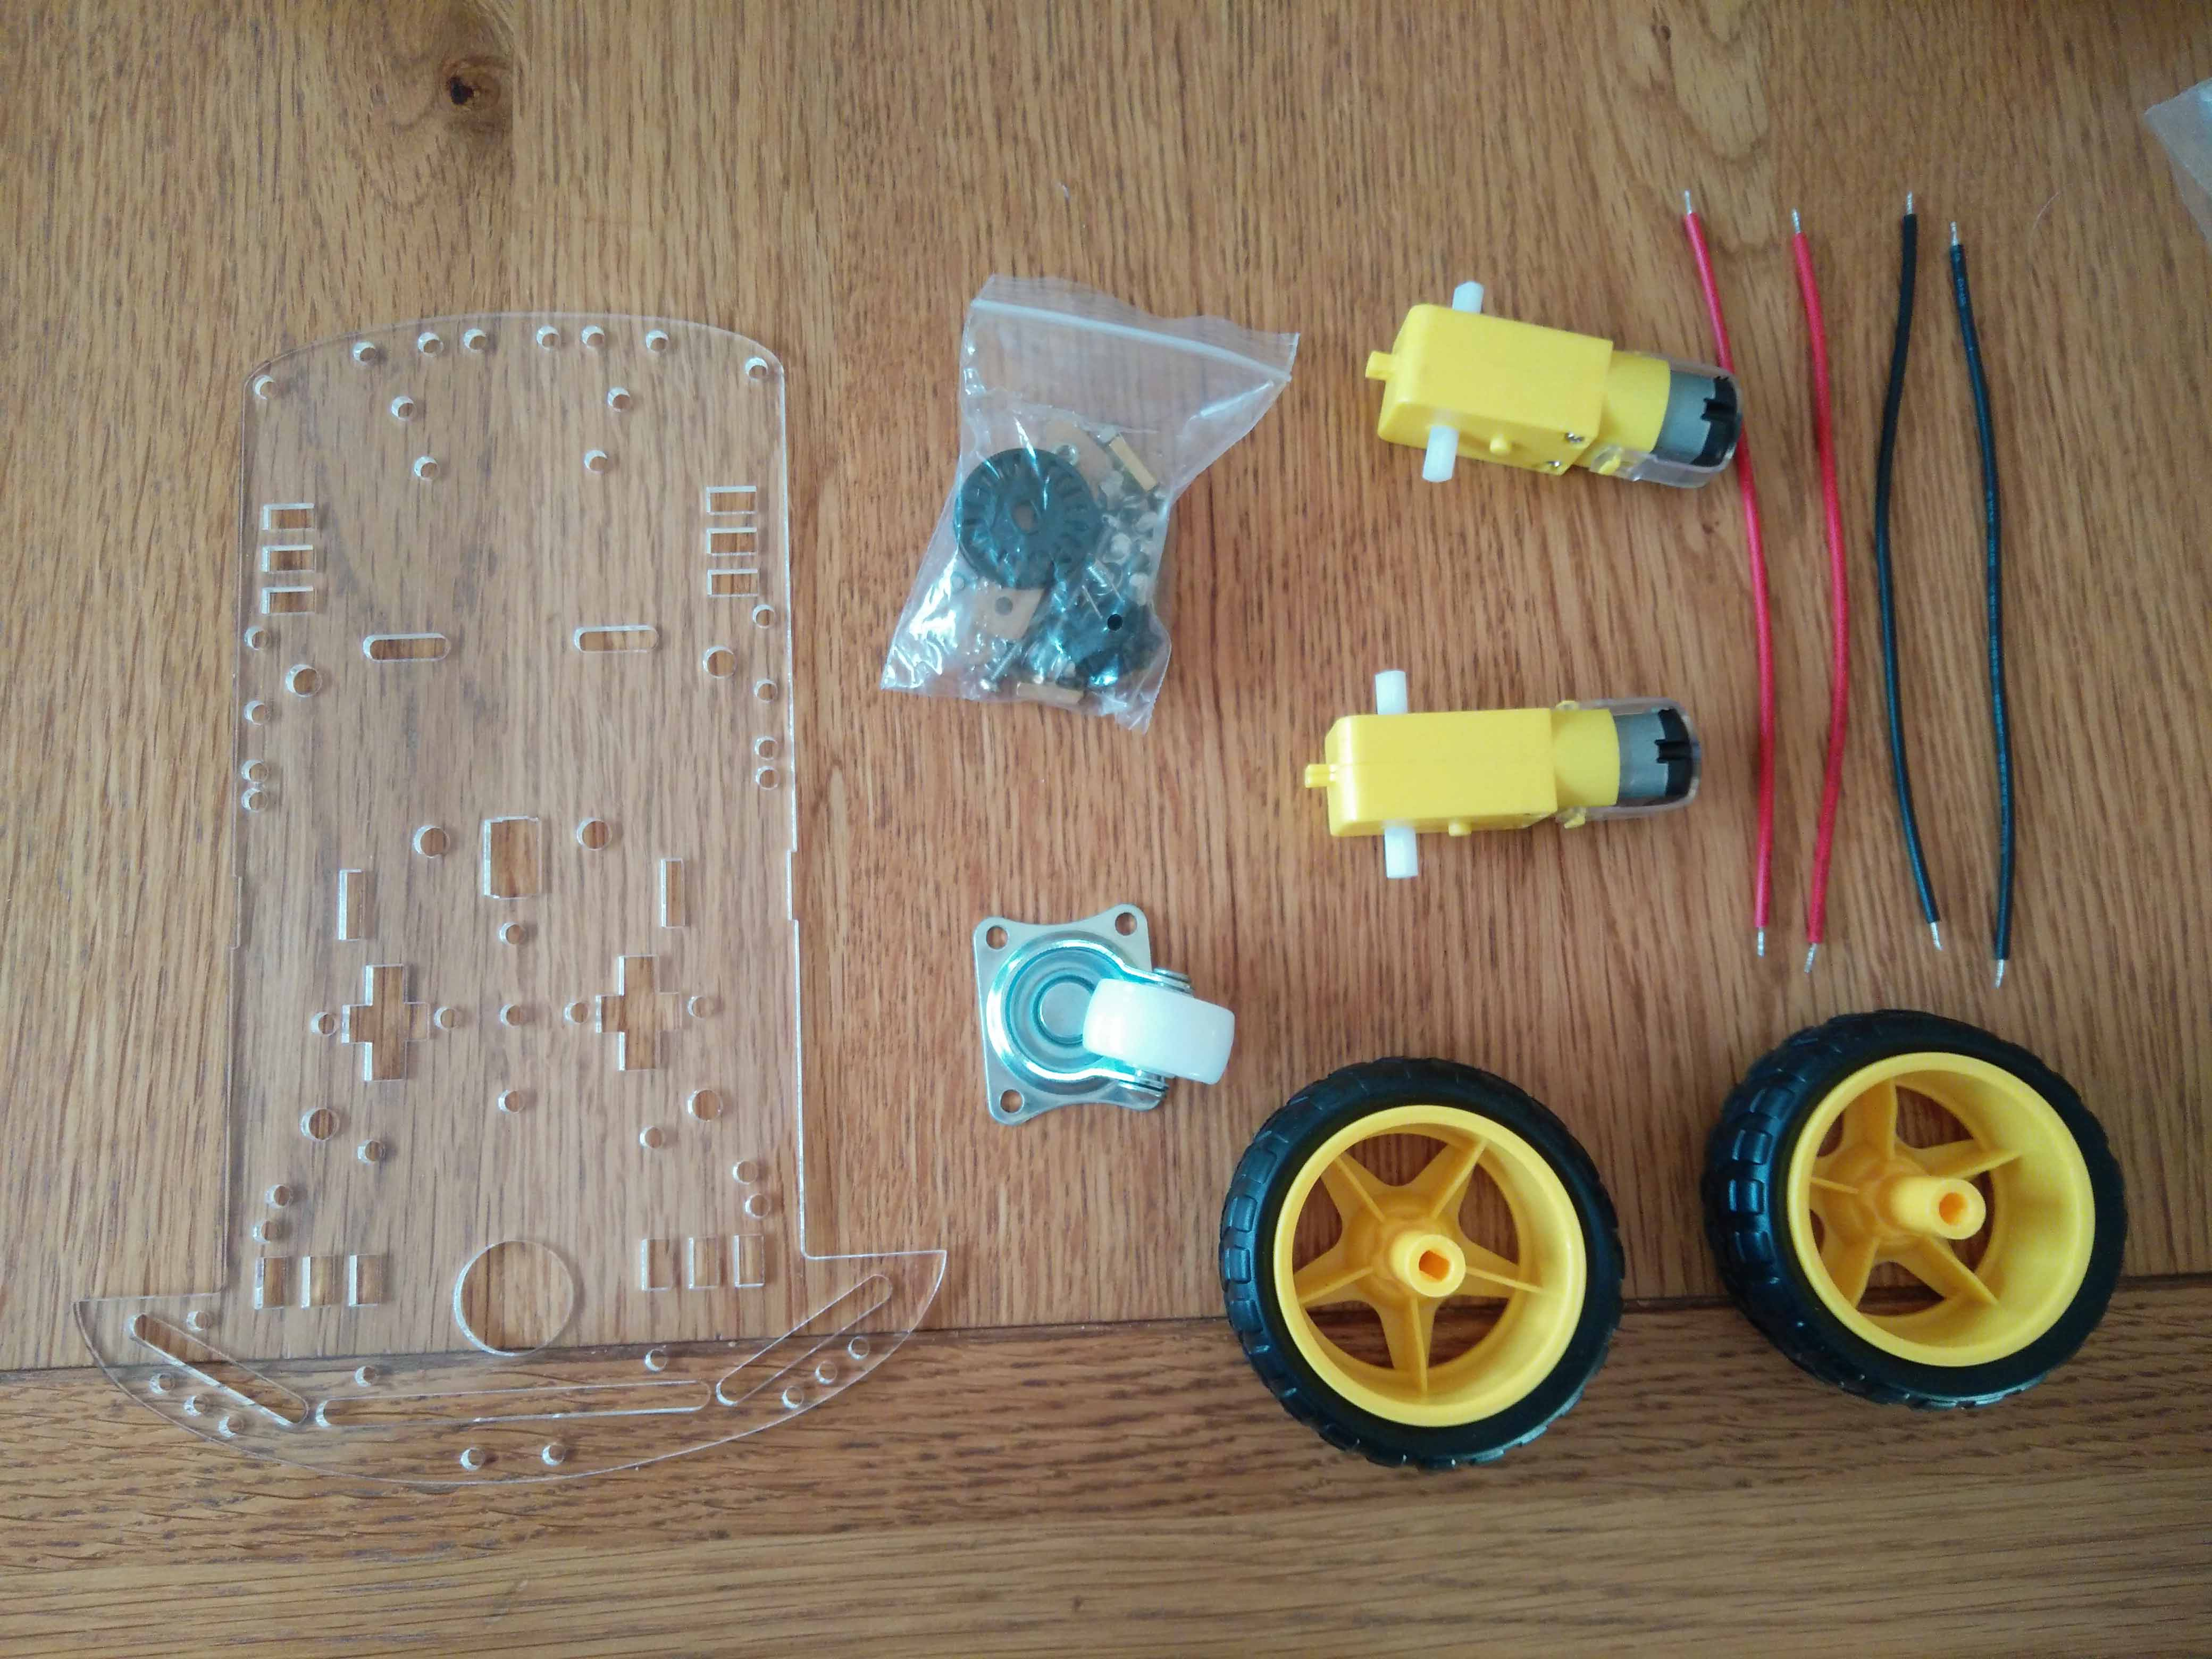
\includegraphics[width=13cm]{img/1.jpg}\par
    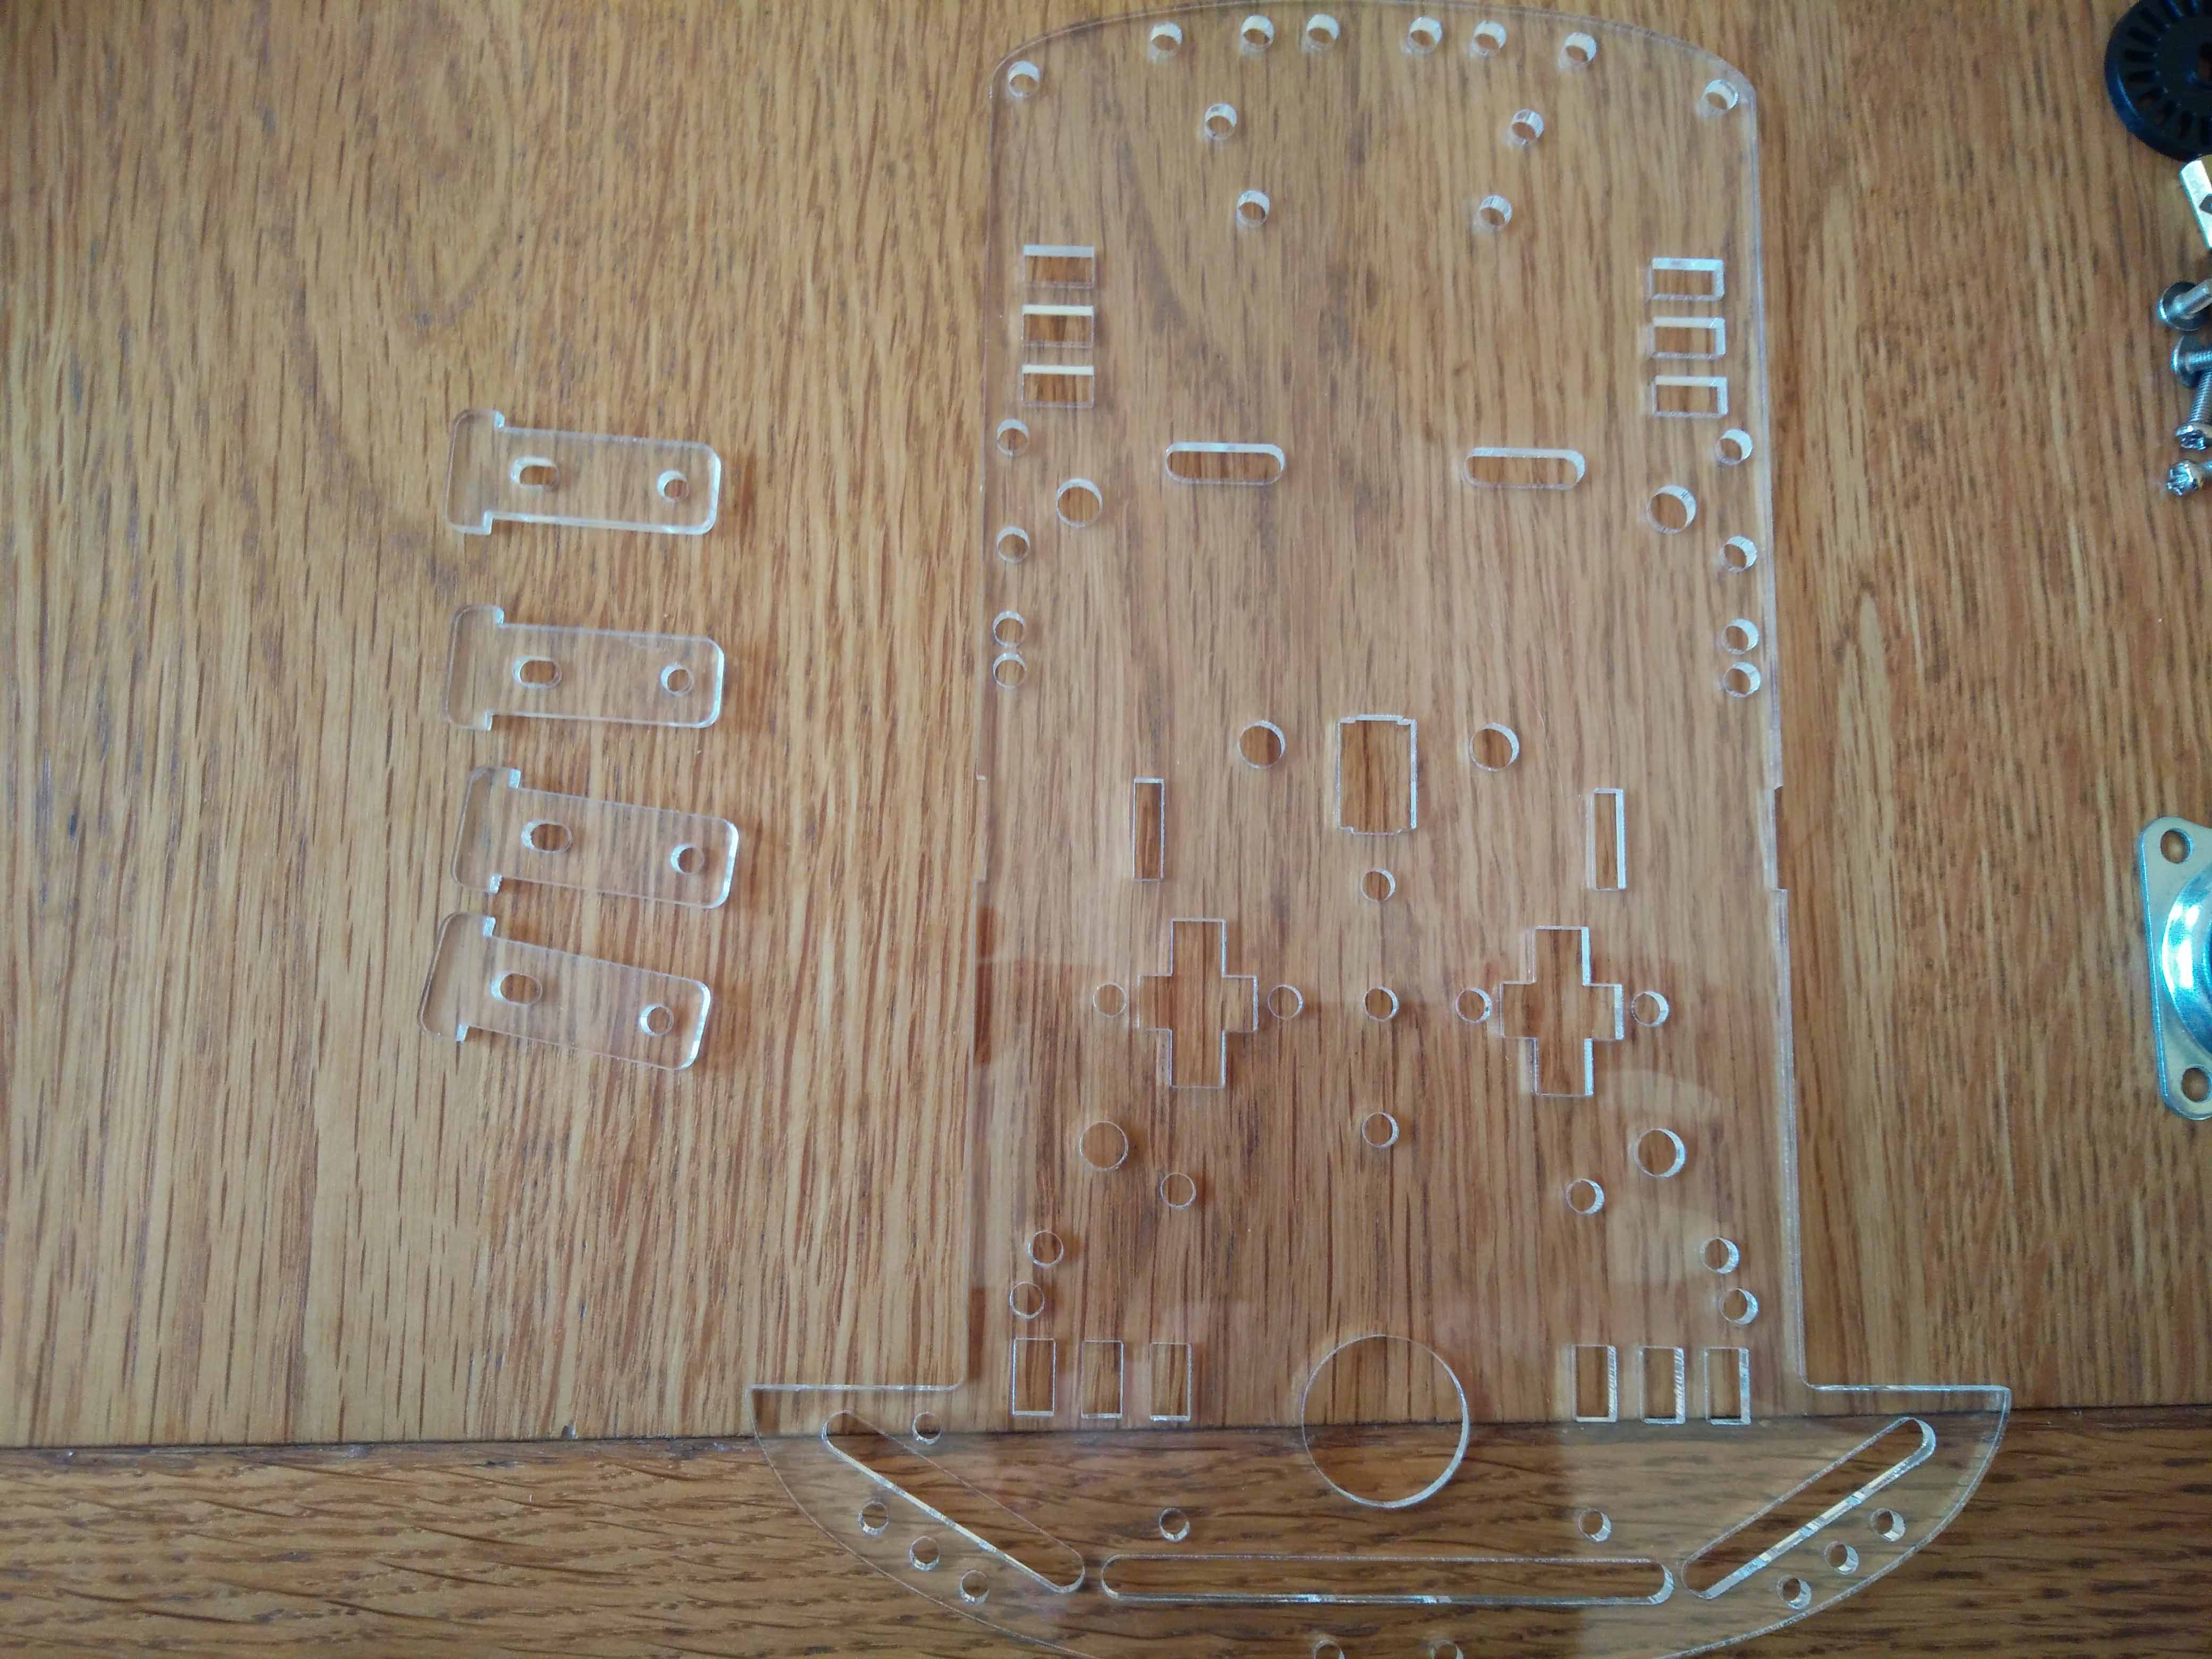
\includegraphics[width=13cm]{img/2.jpg}\par
    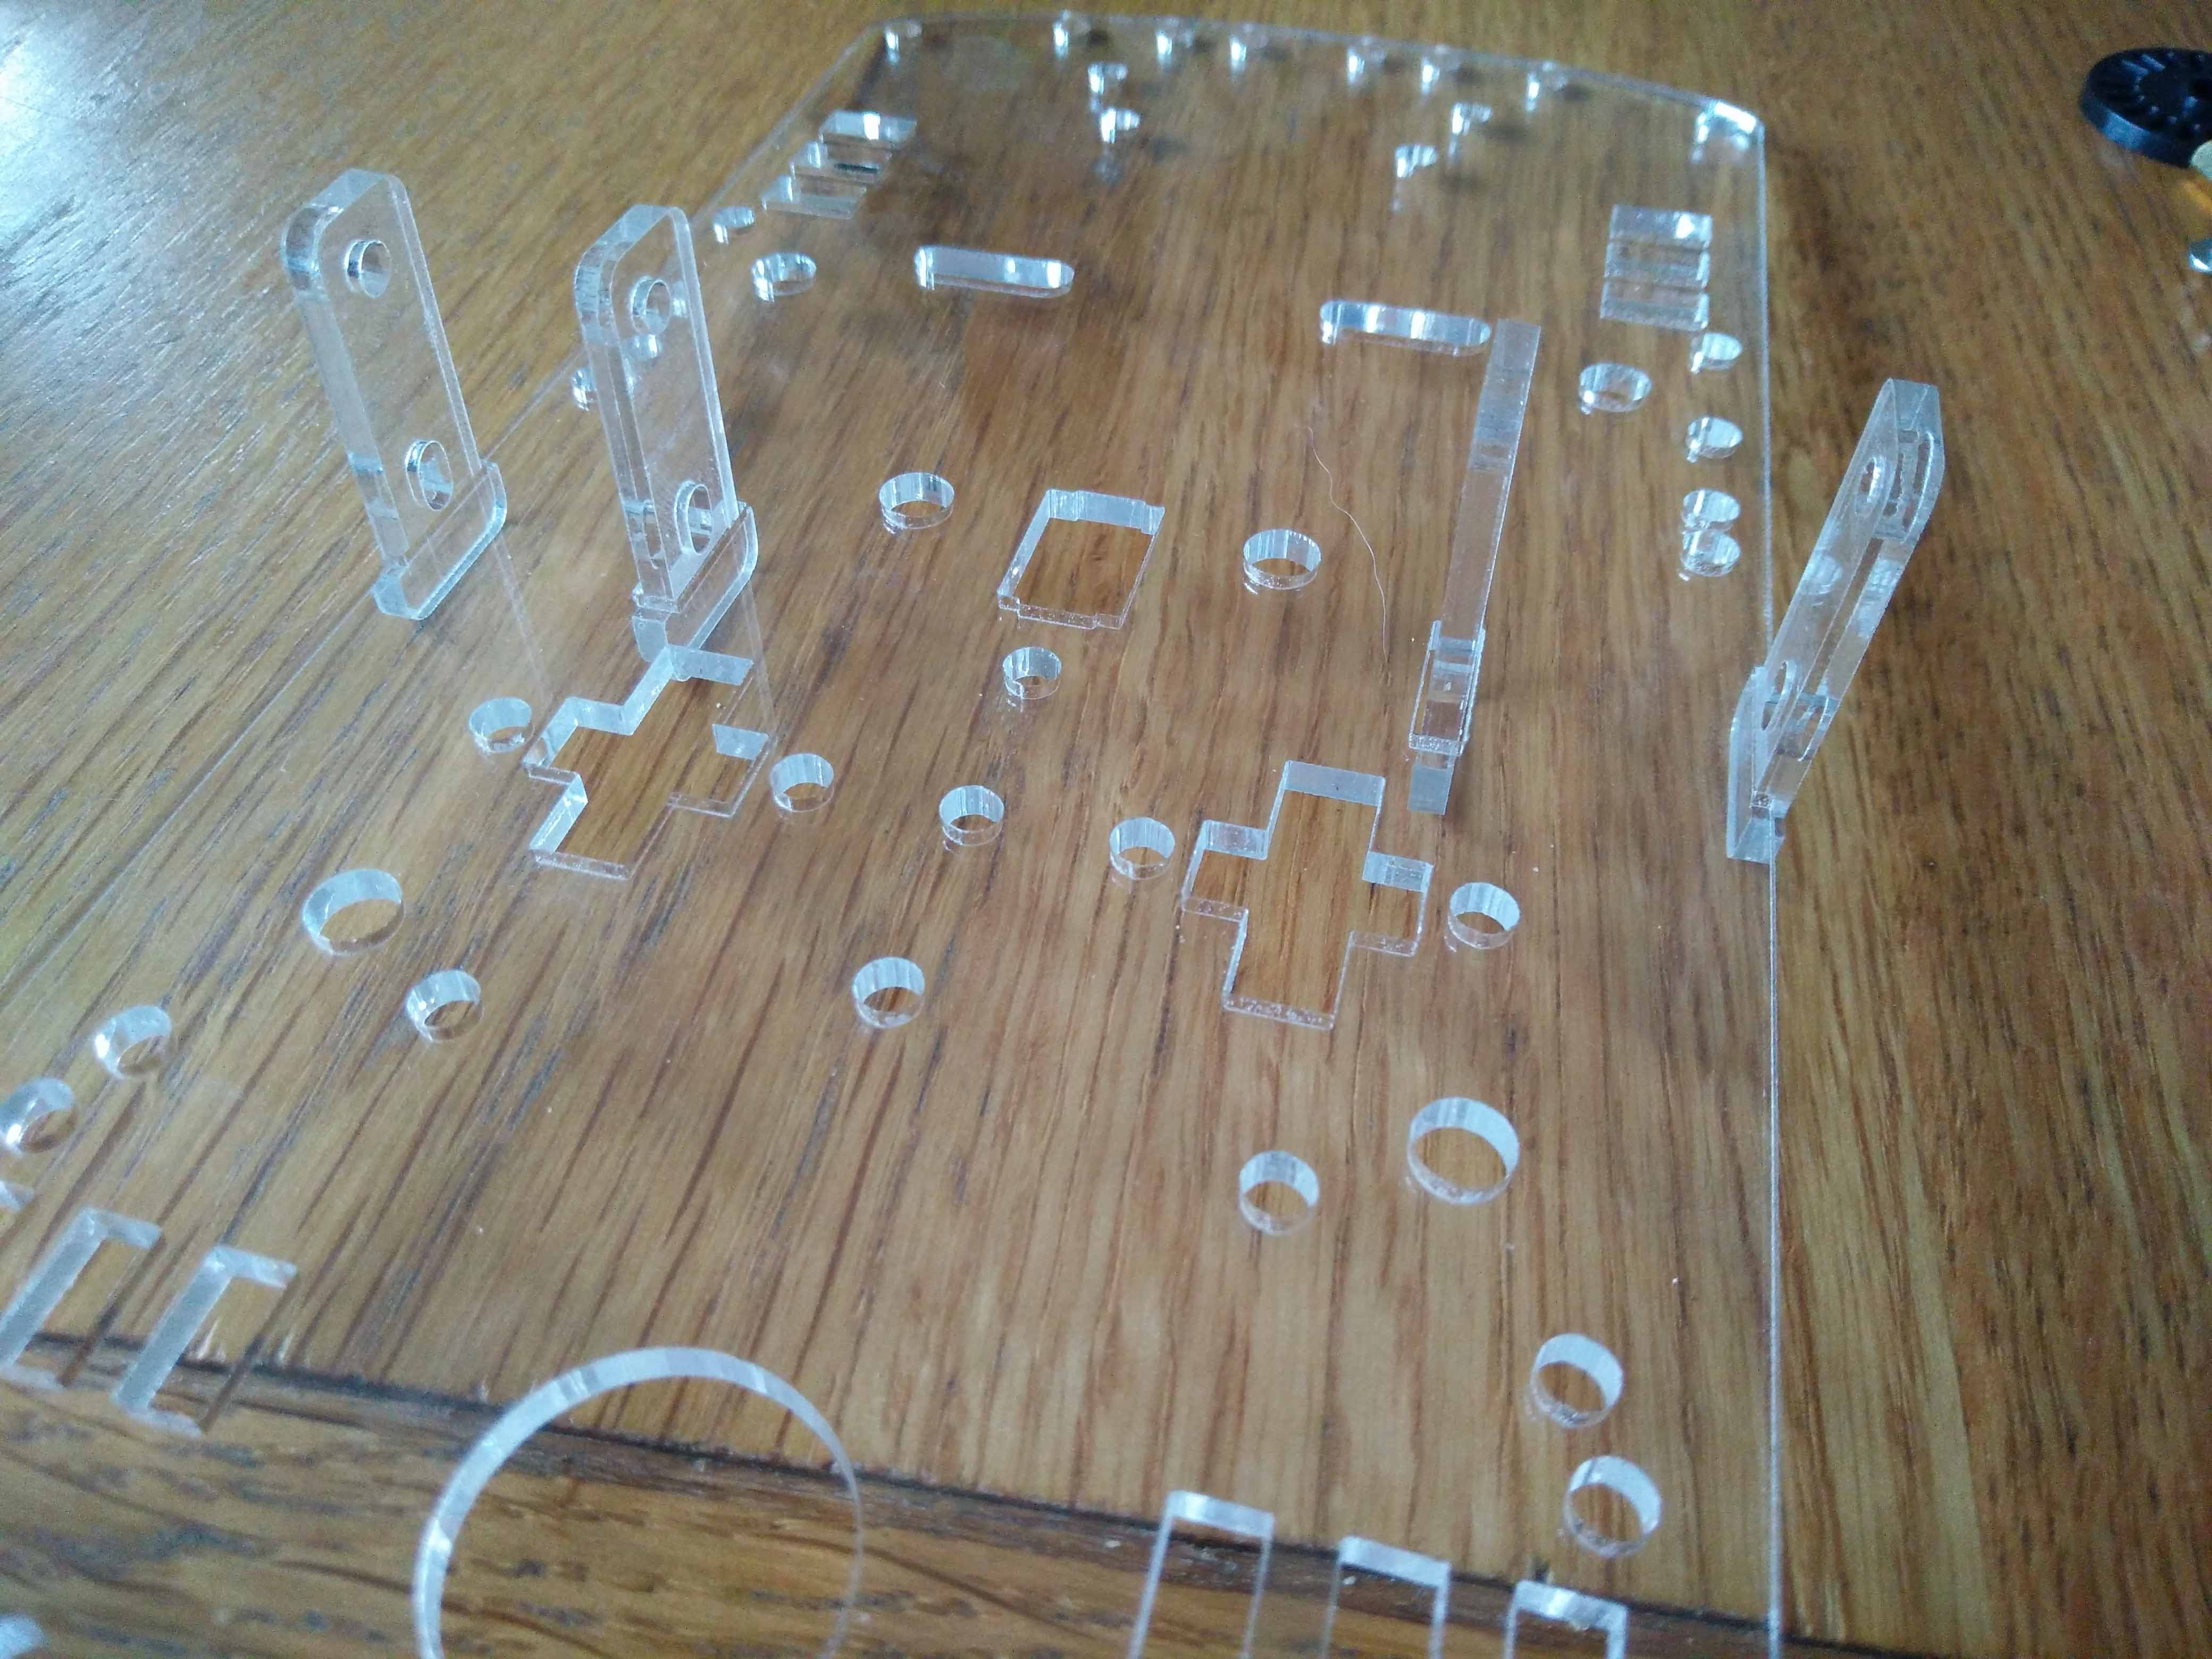
\includegraphics[width=15cm]{img/3.jpg}\par
    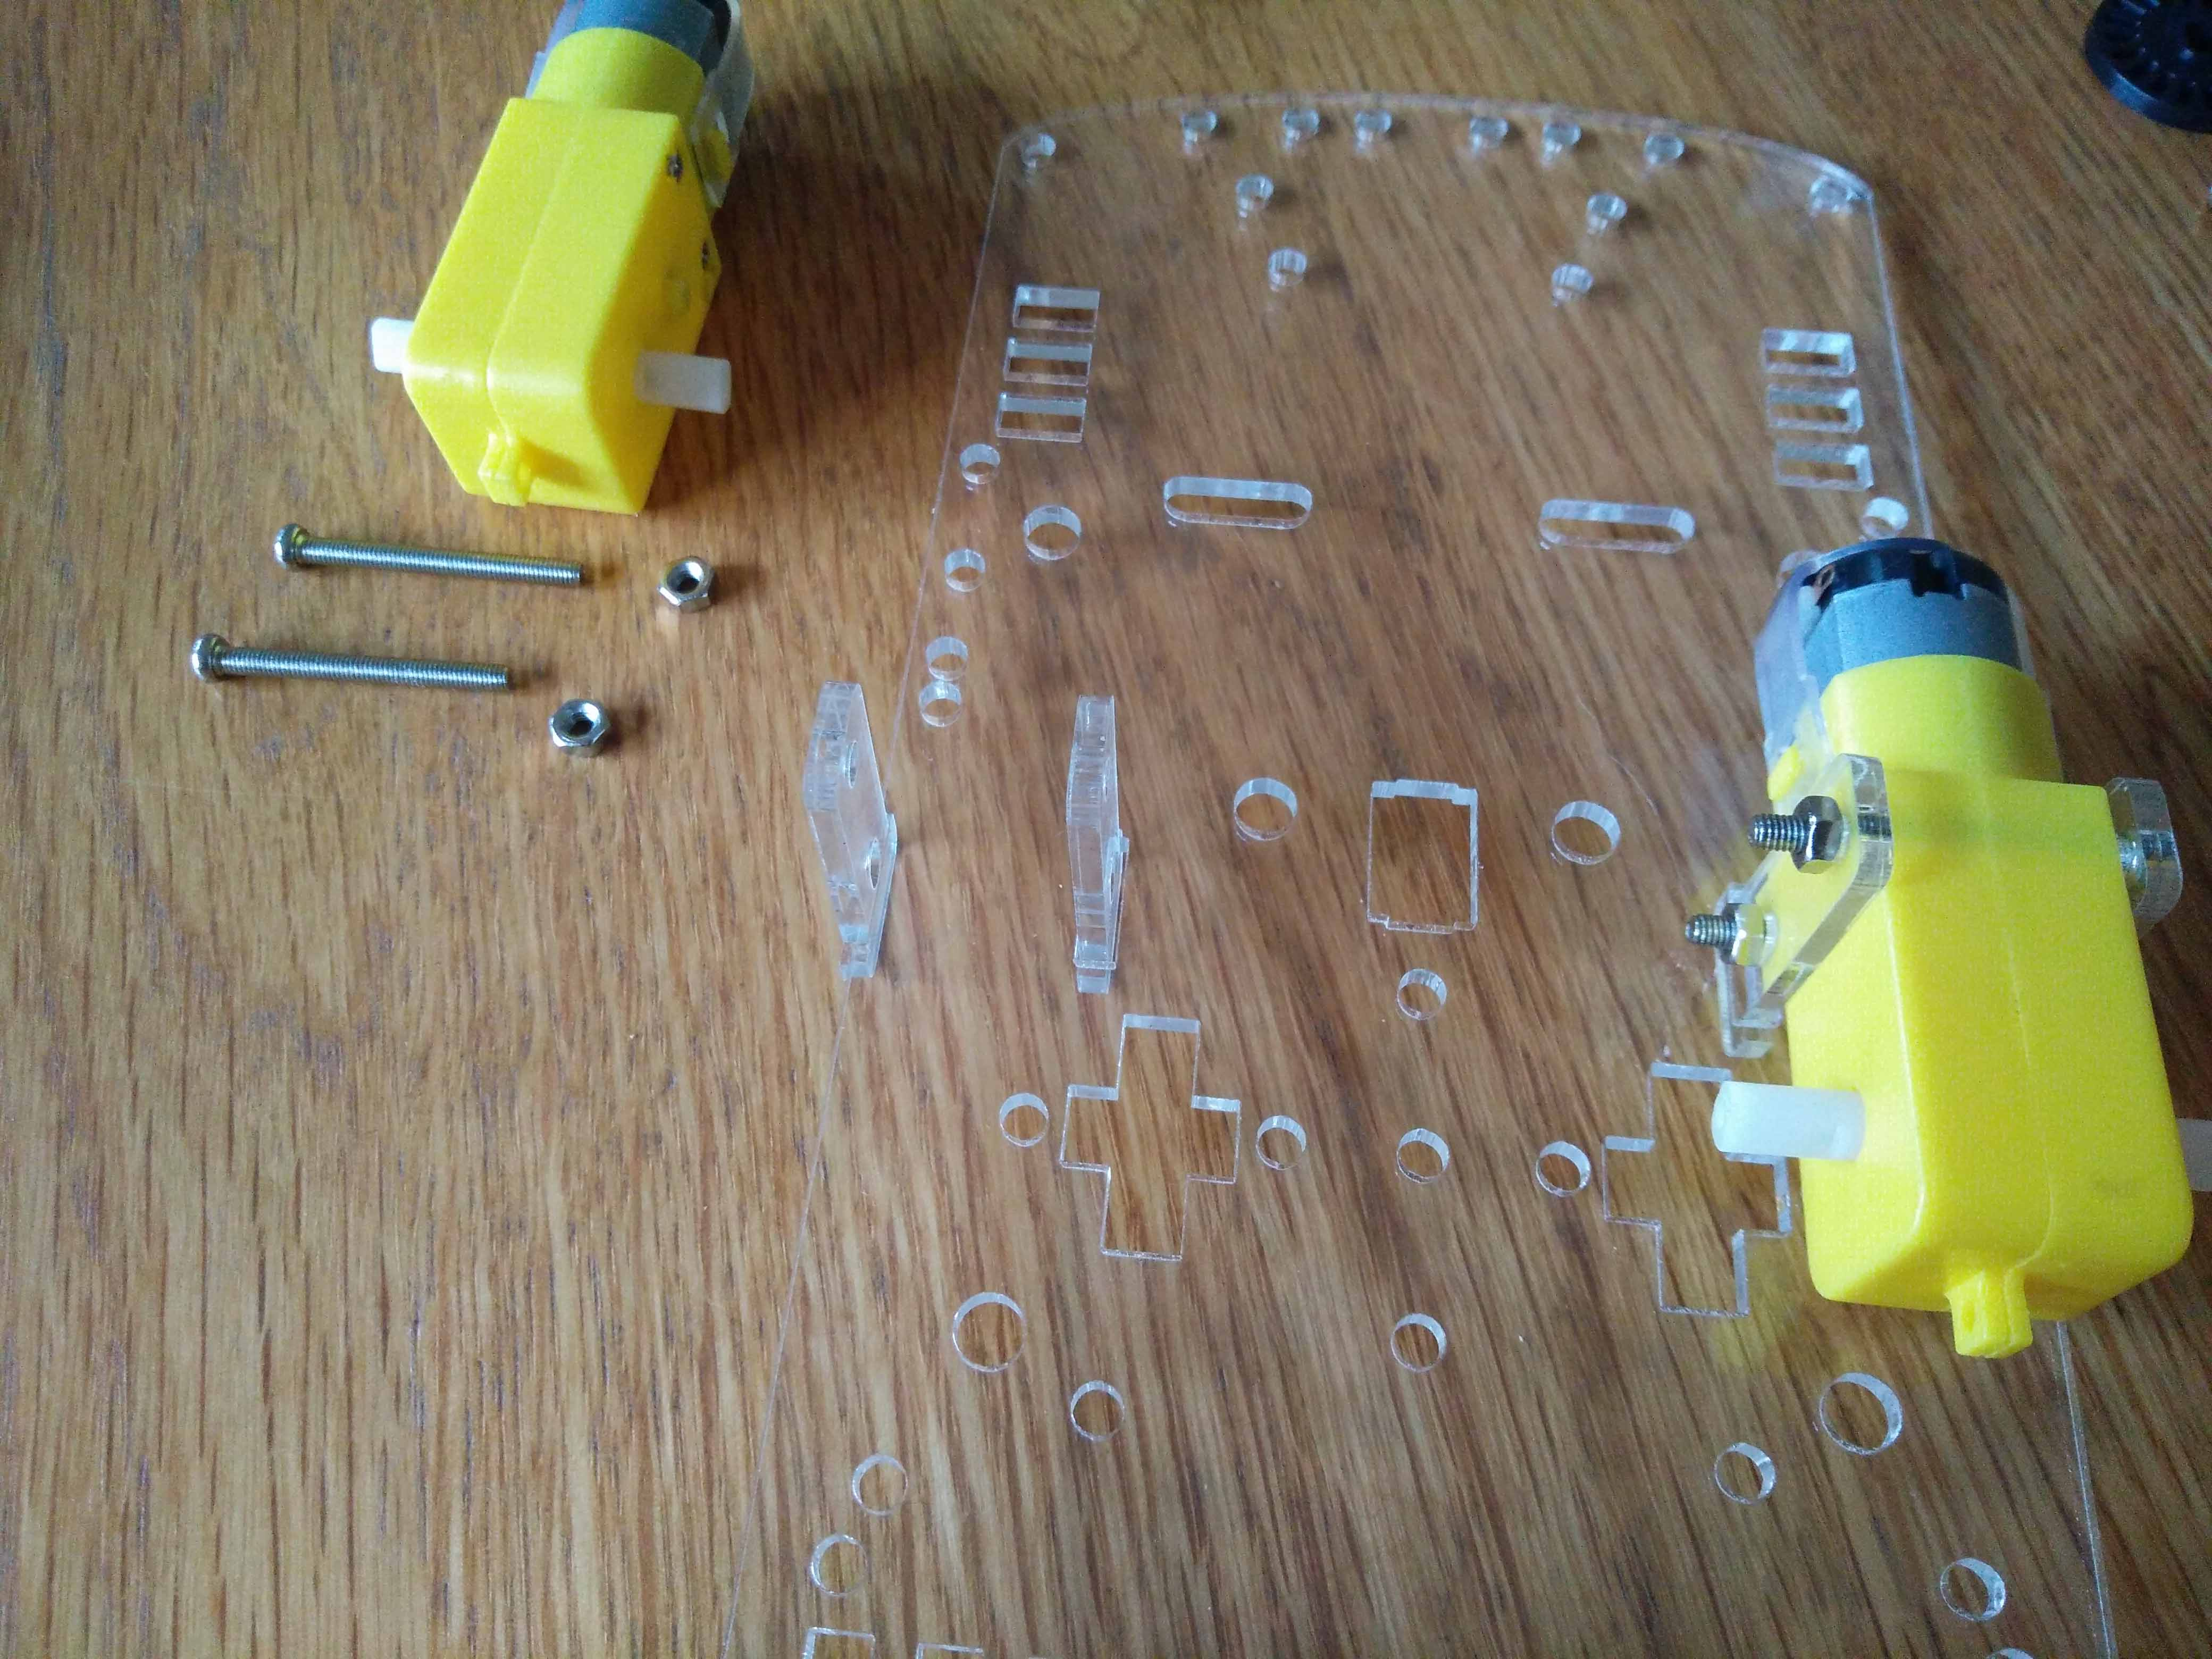
\includegraphics[width=15cm]{img/4.jpg}\par
    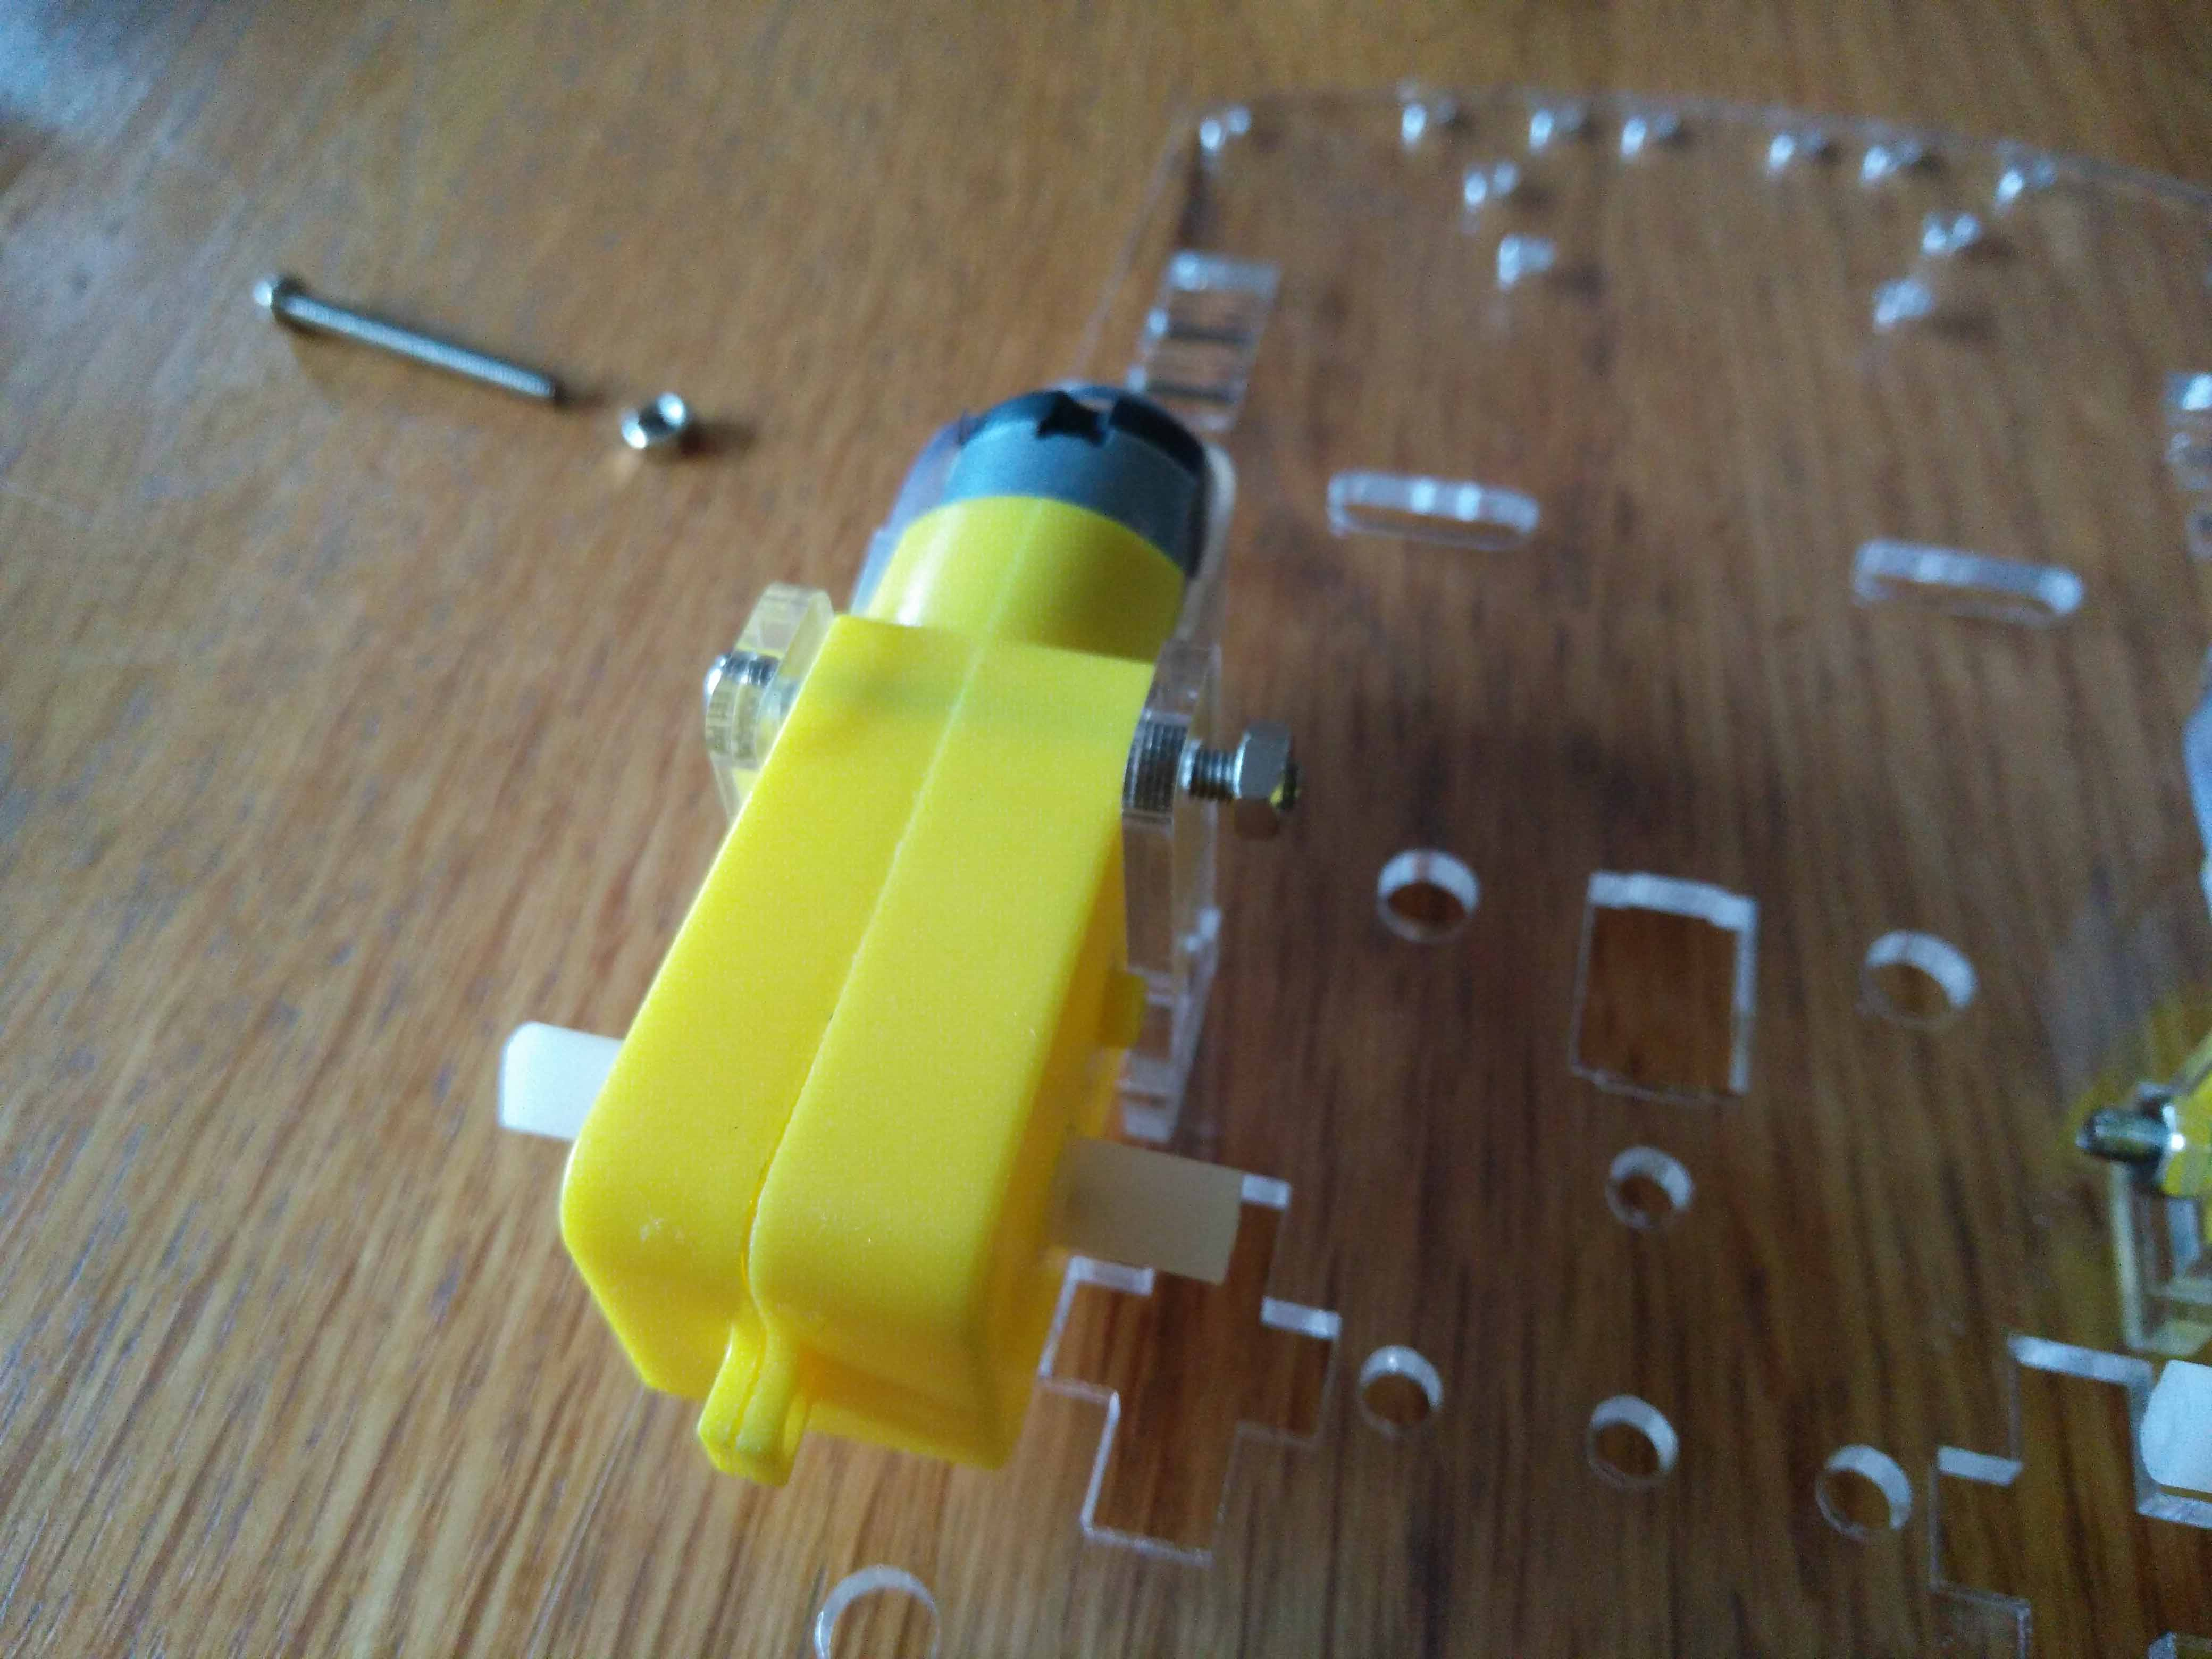
\includegraphics[width=15cm]{img/5.jpg}\par
    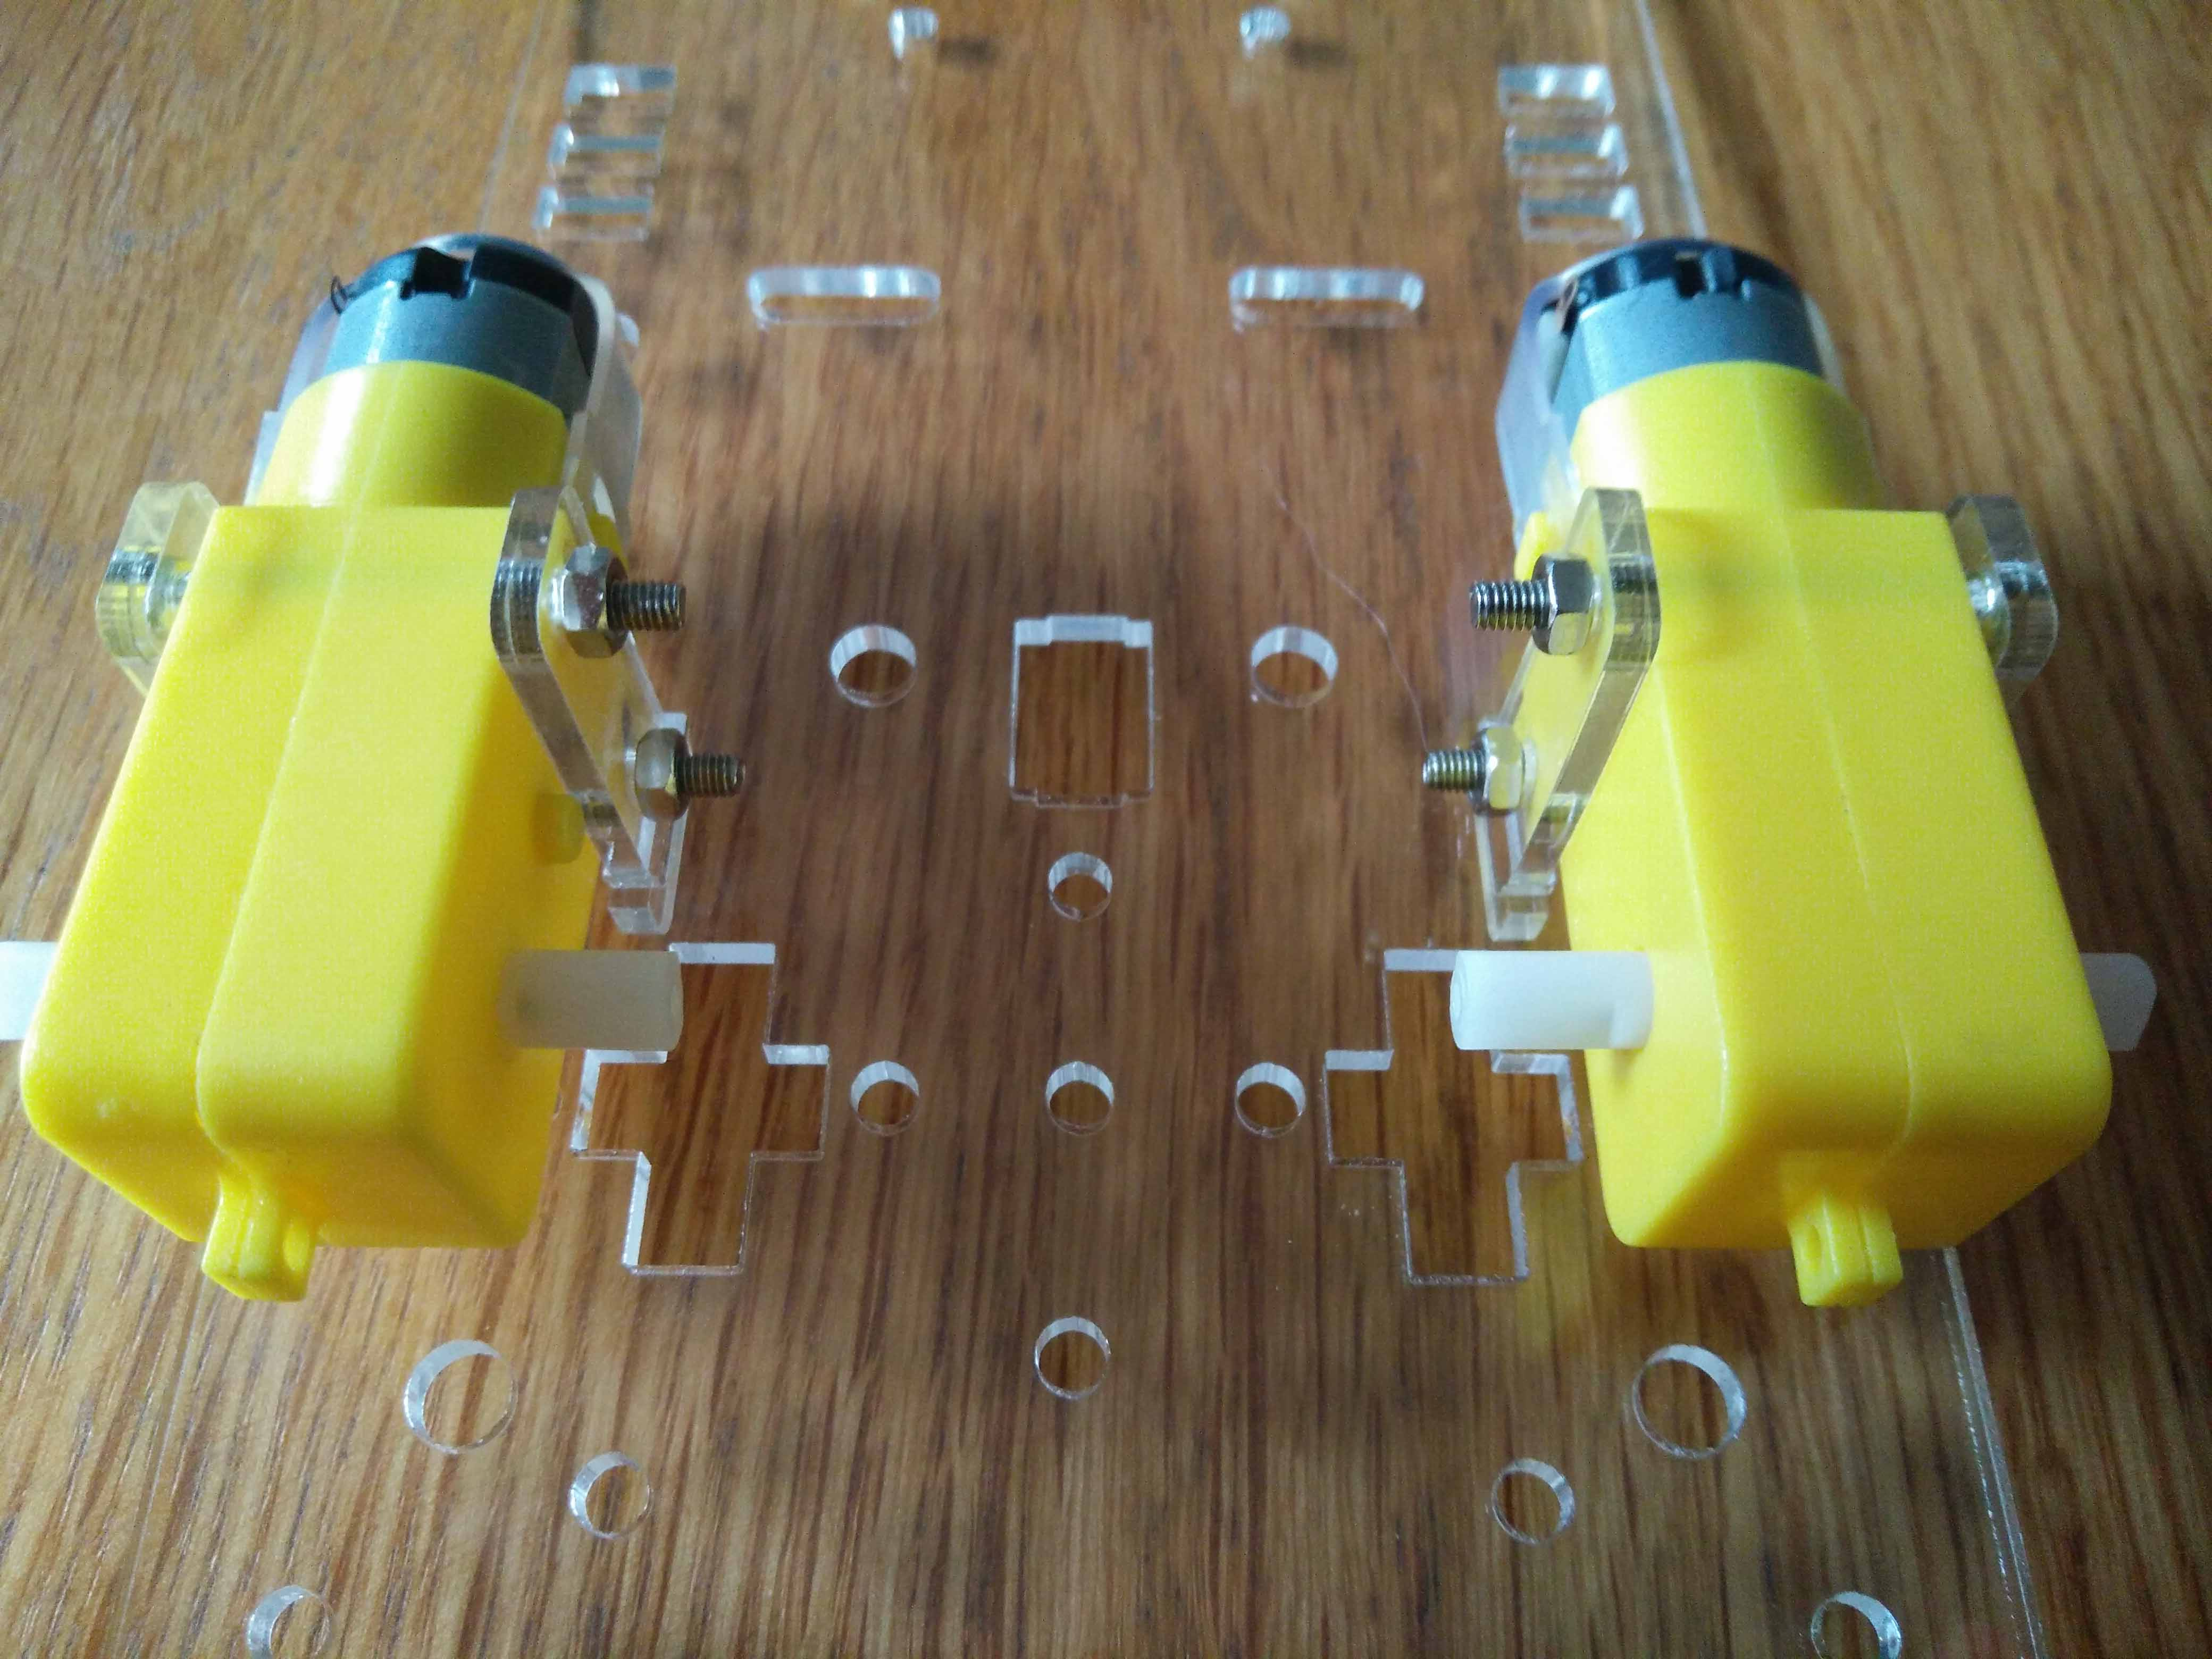
\includegraphics[width=15cm]{img/6.jpg}\par
    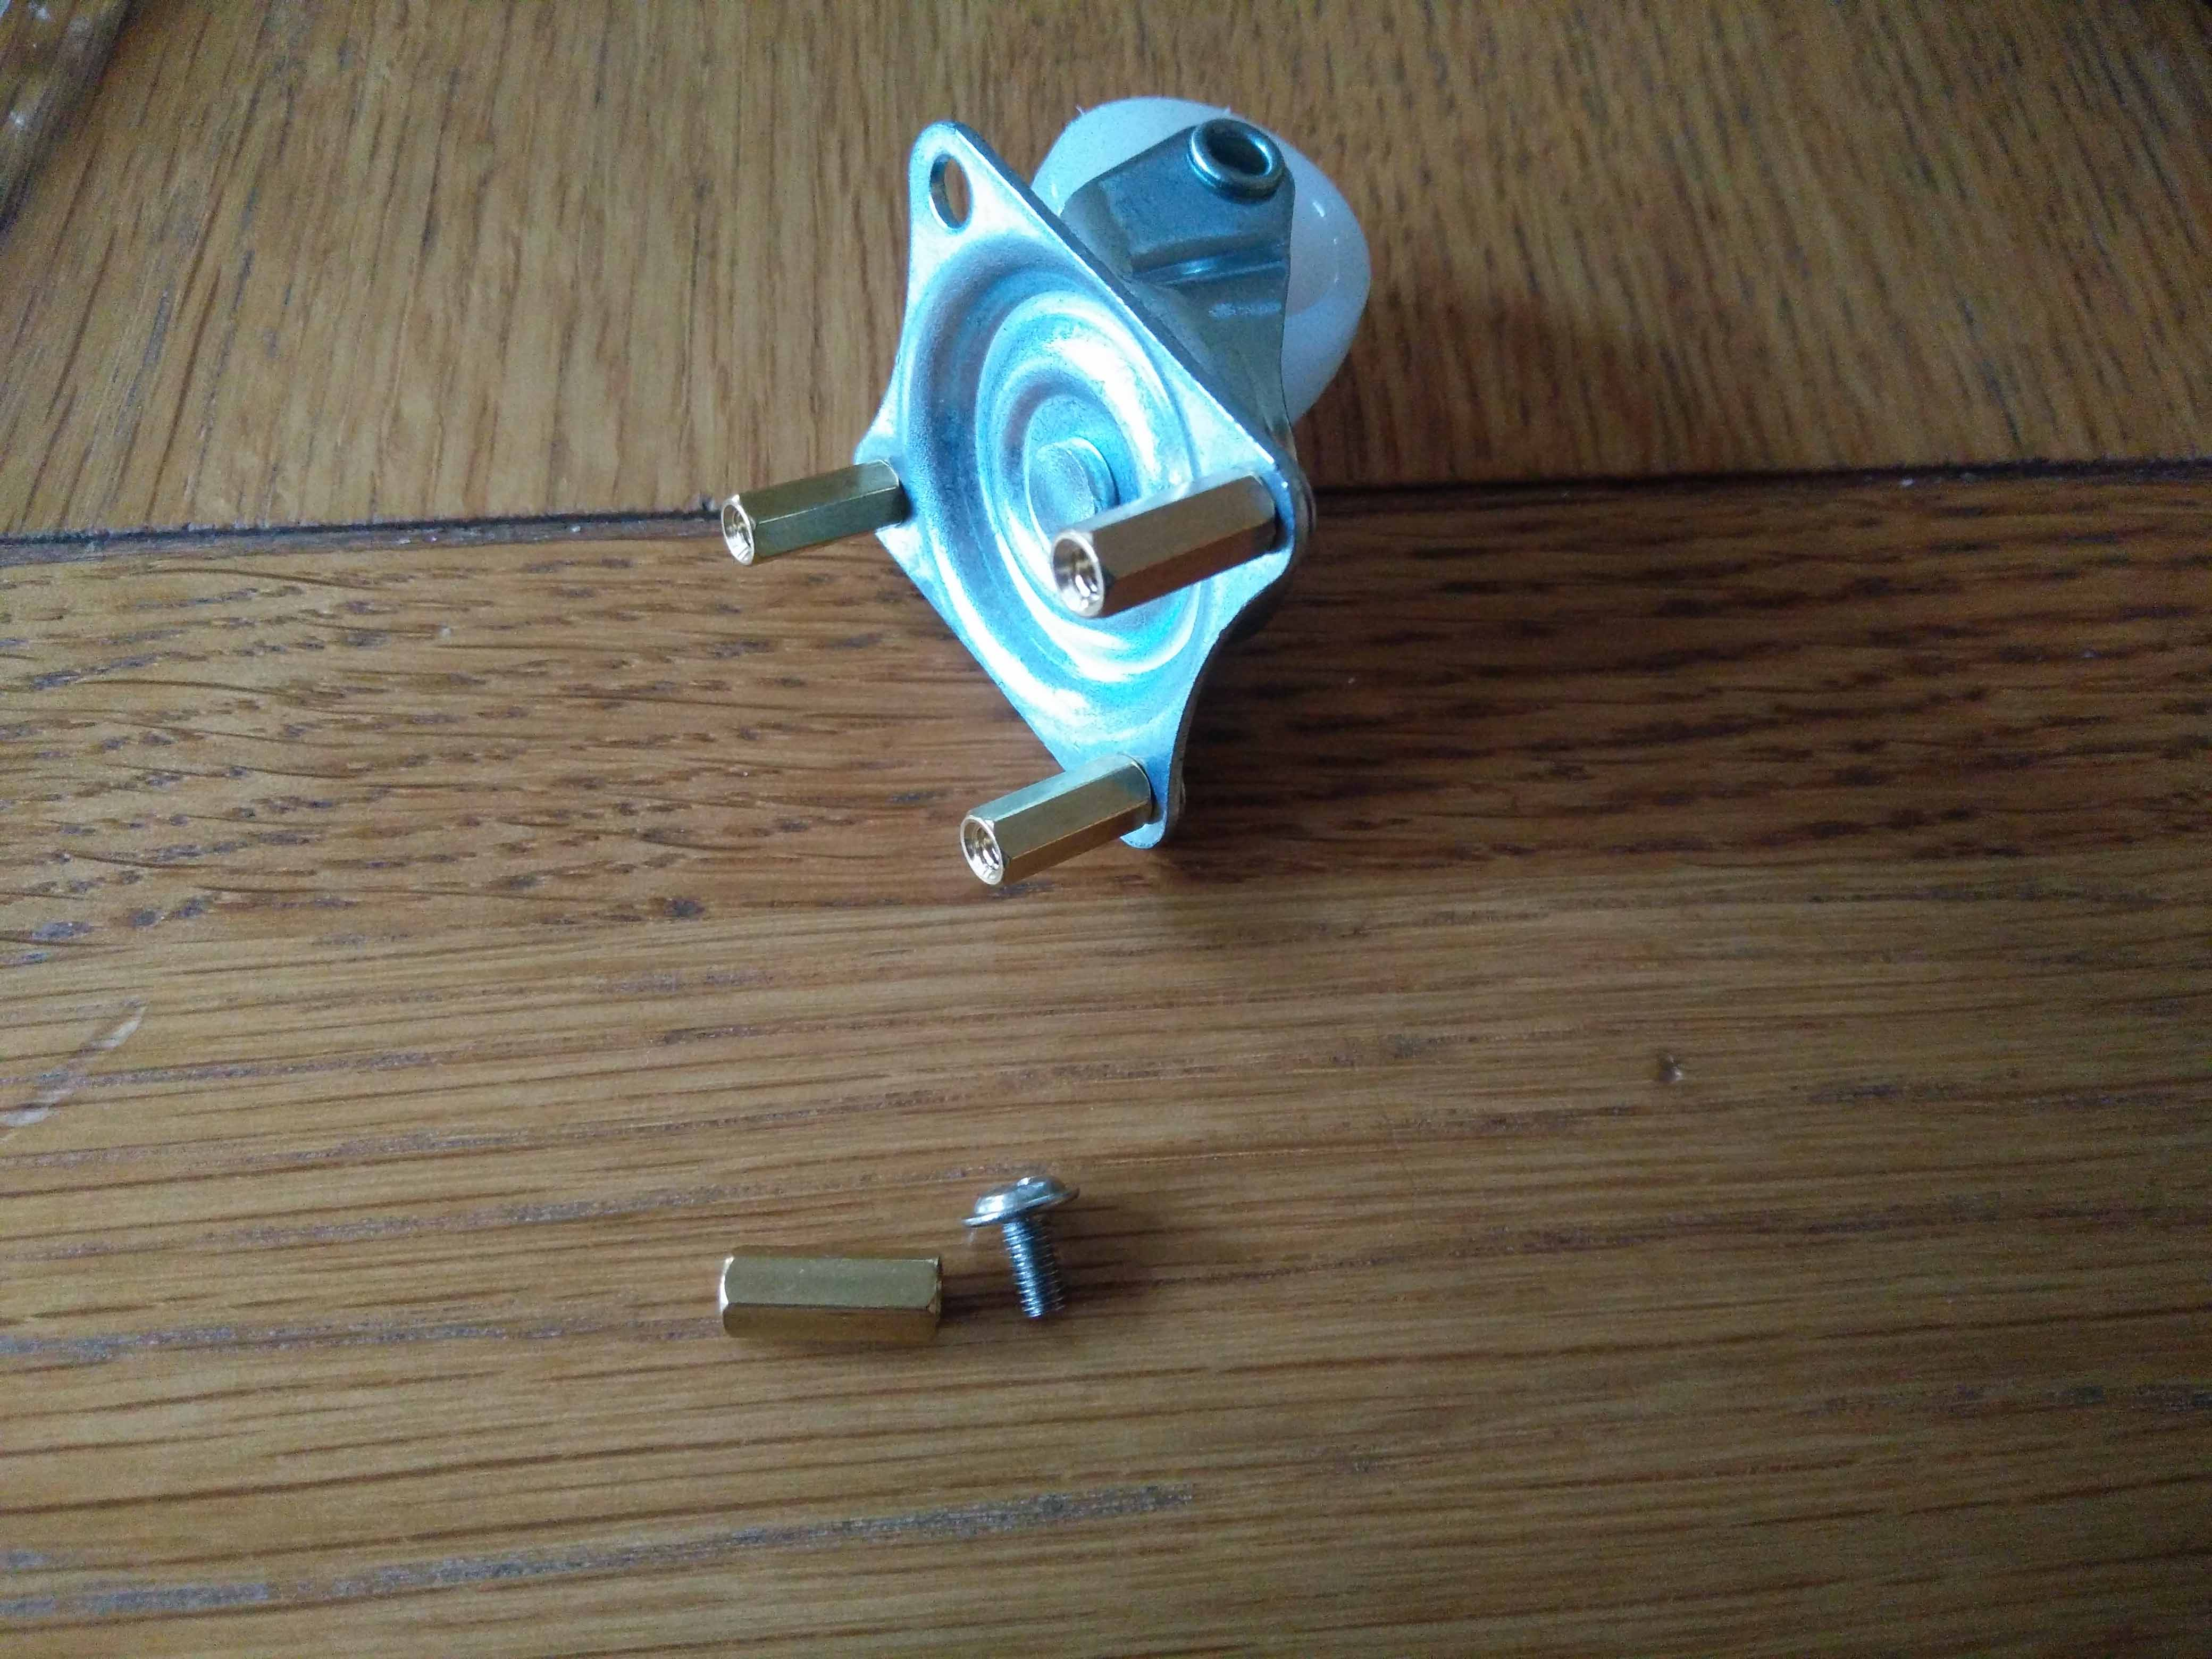
\includegraphics[width=15cm]{img/7.jpg}\par
    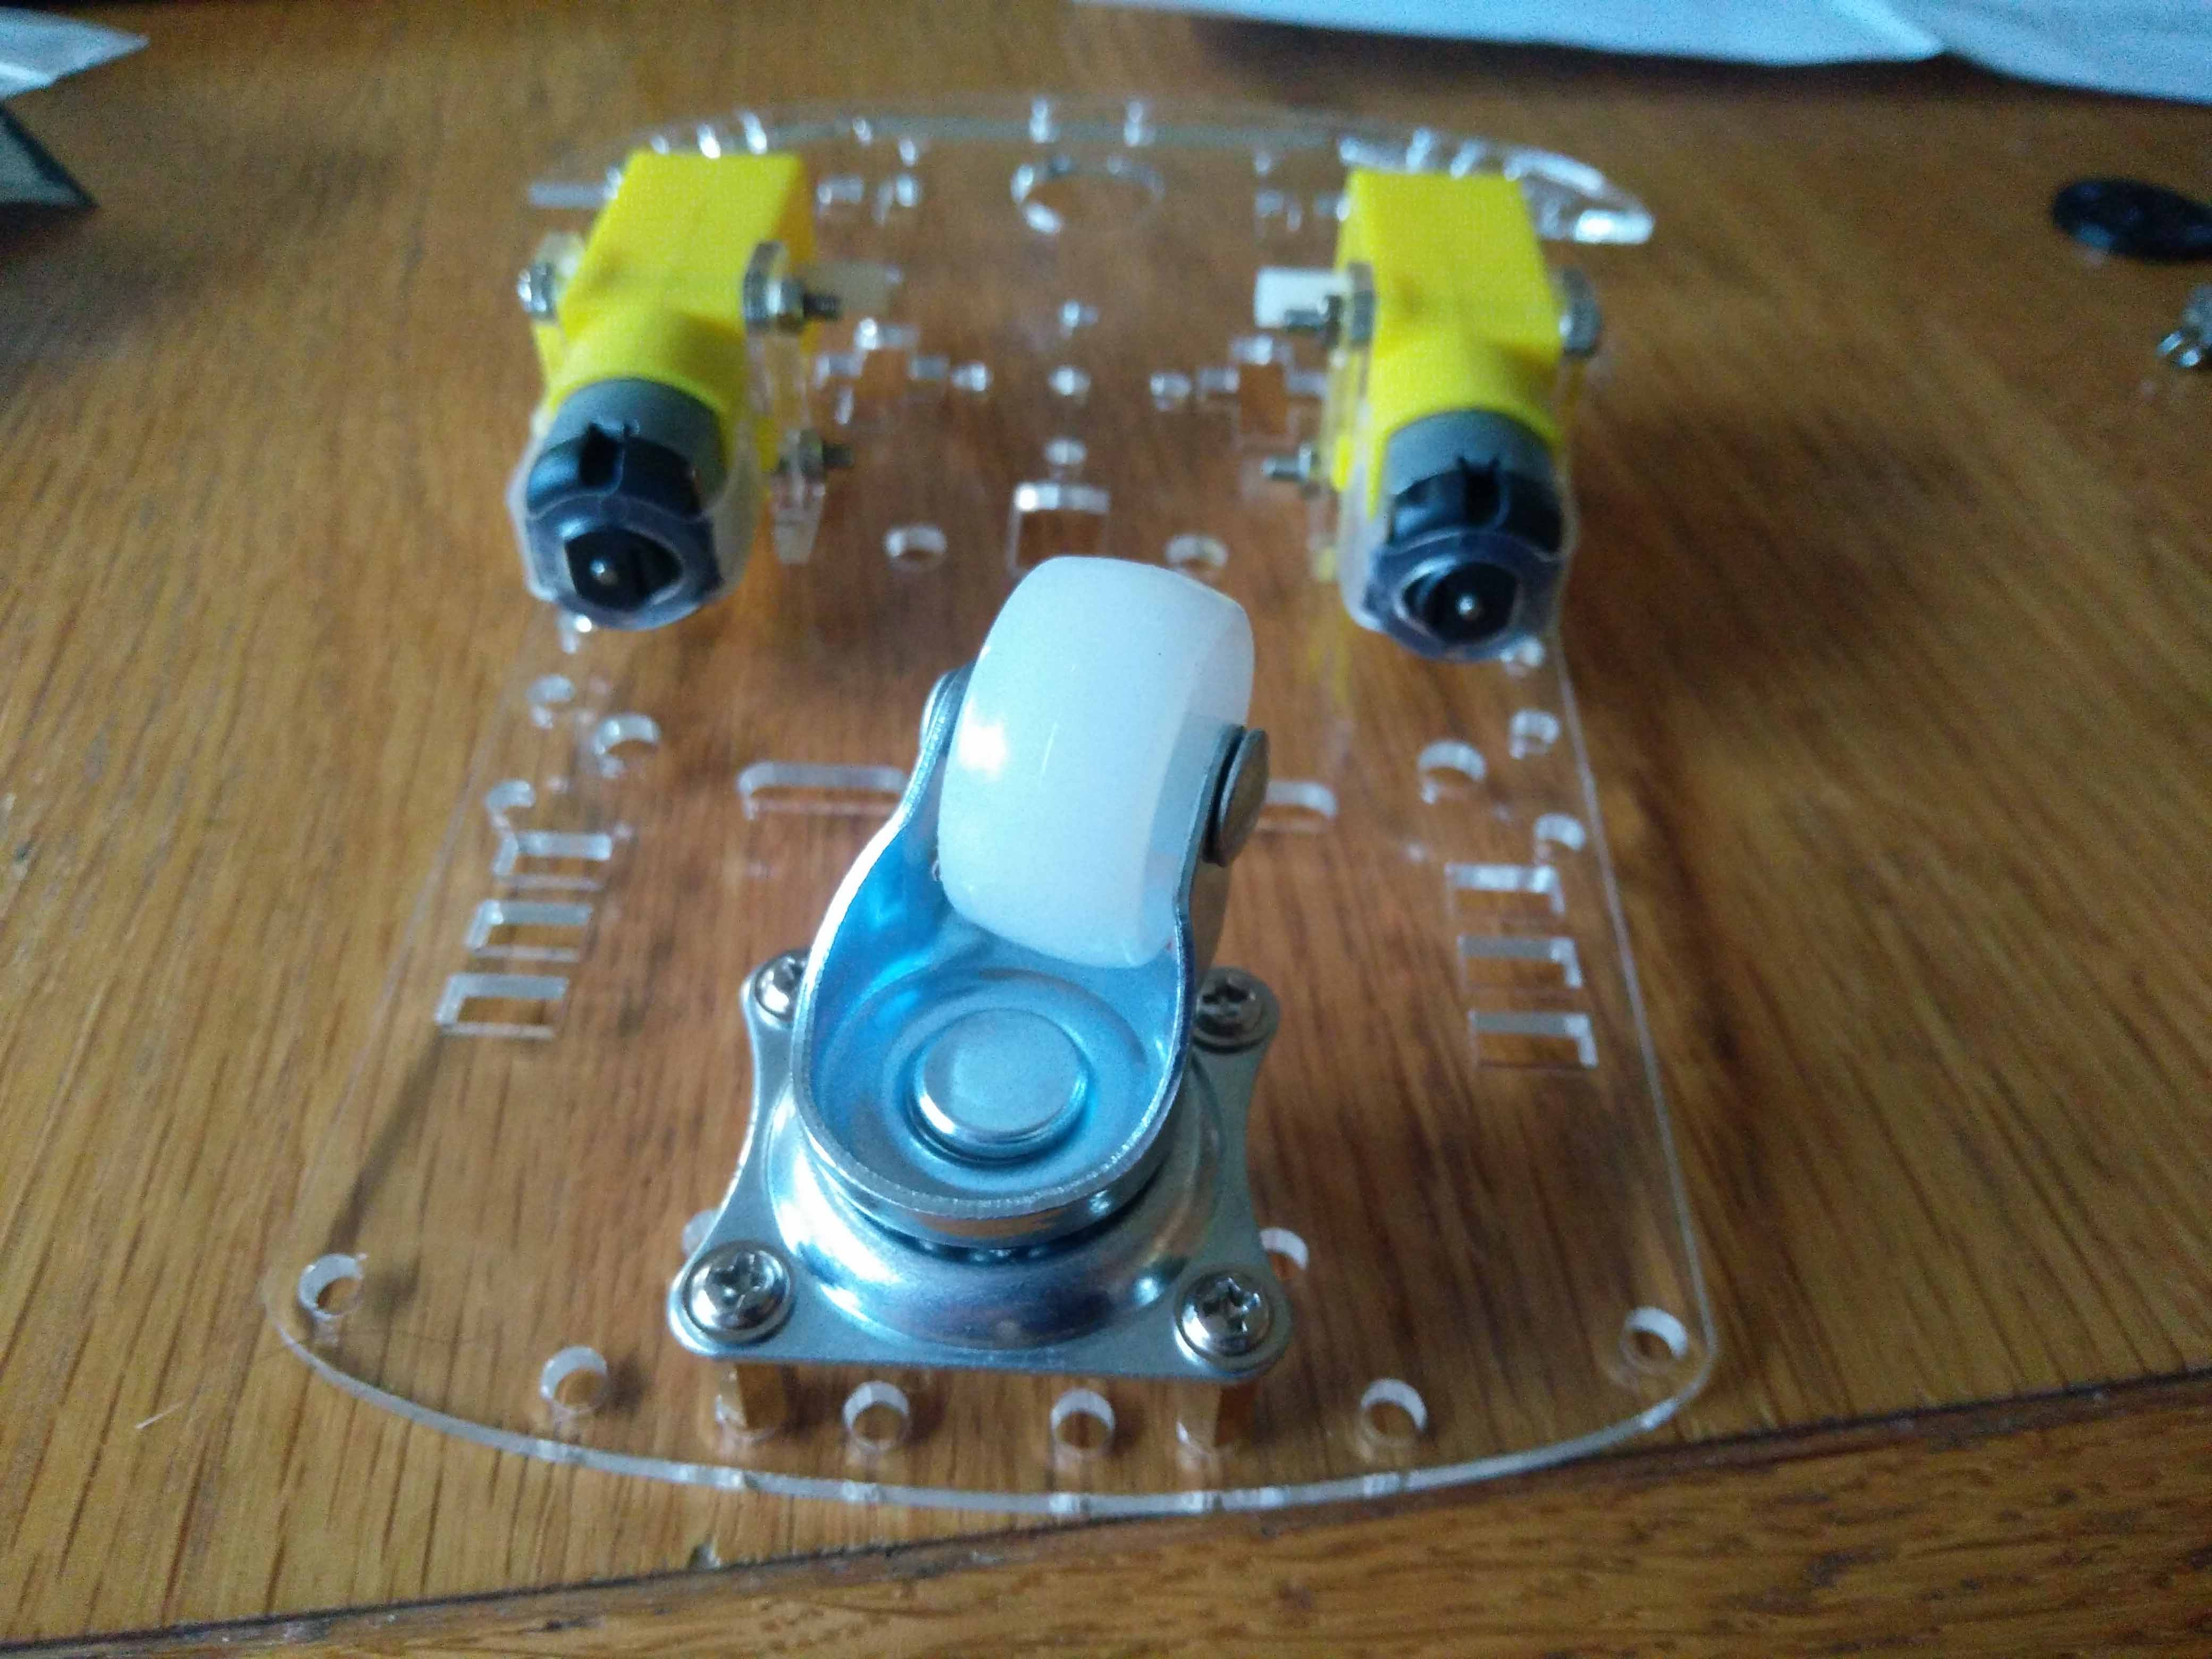
\includegraphics[width=15cm]{img/8.jpg}\par
    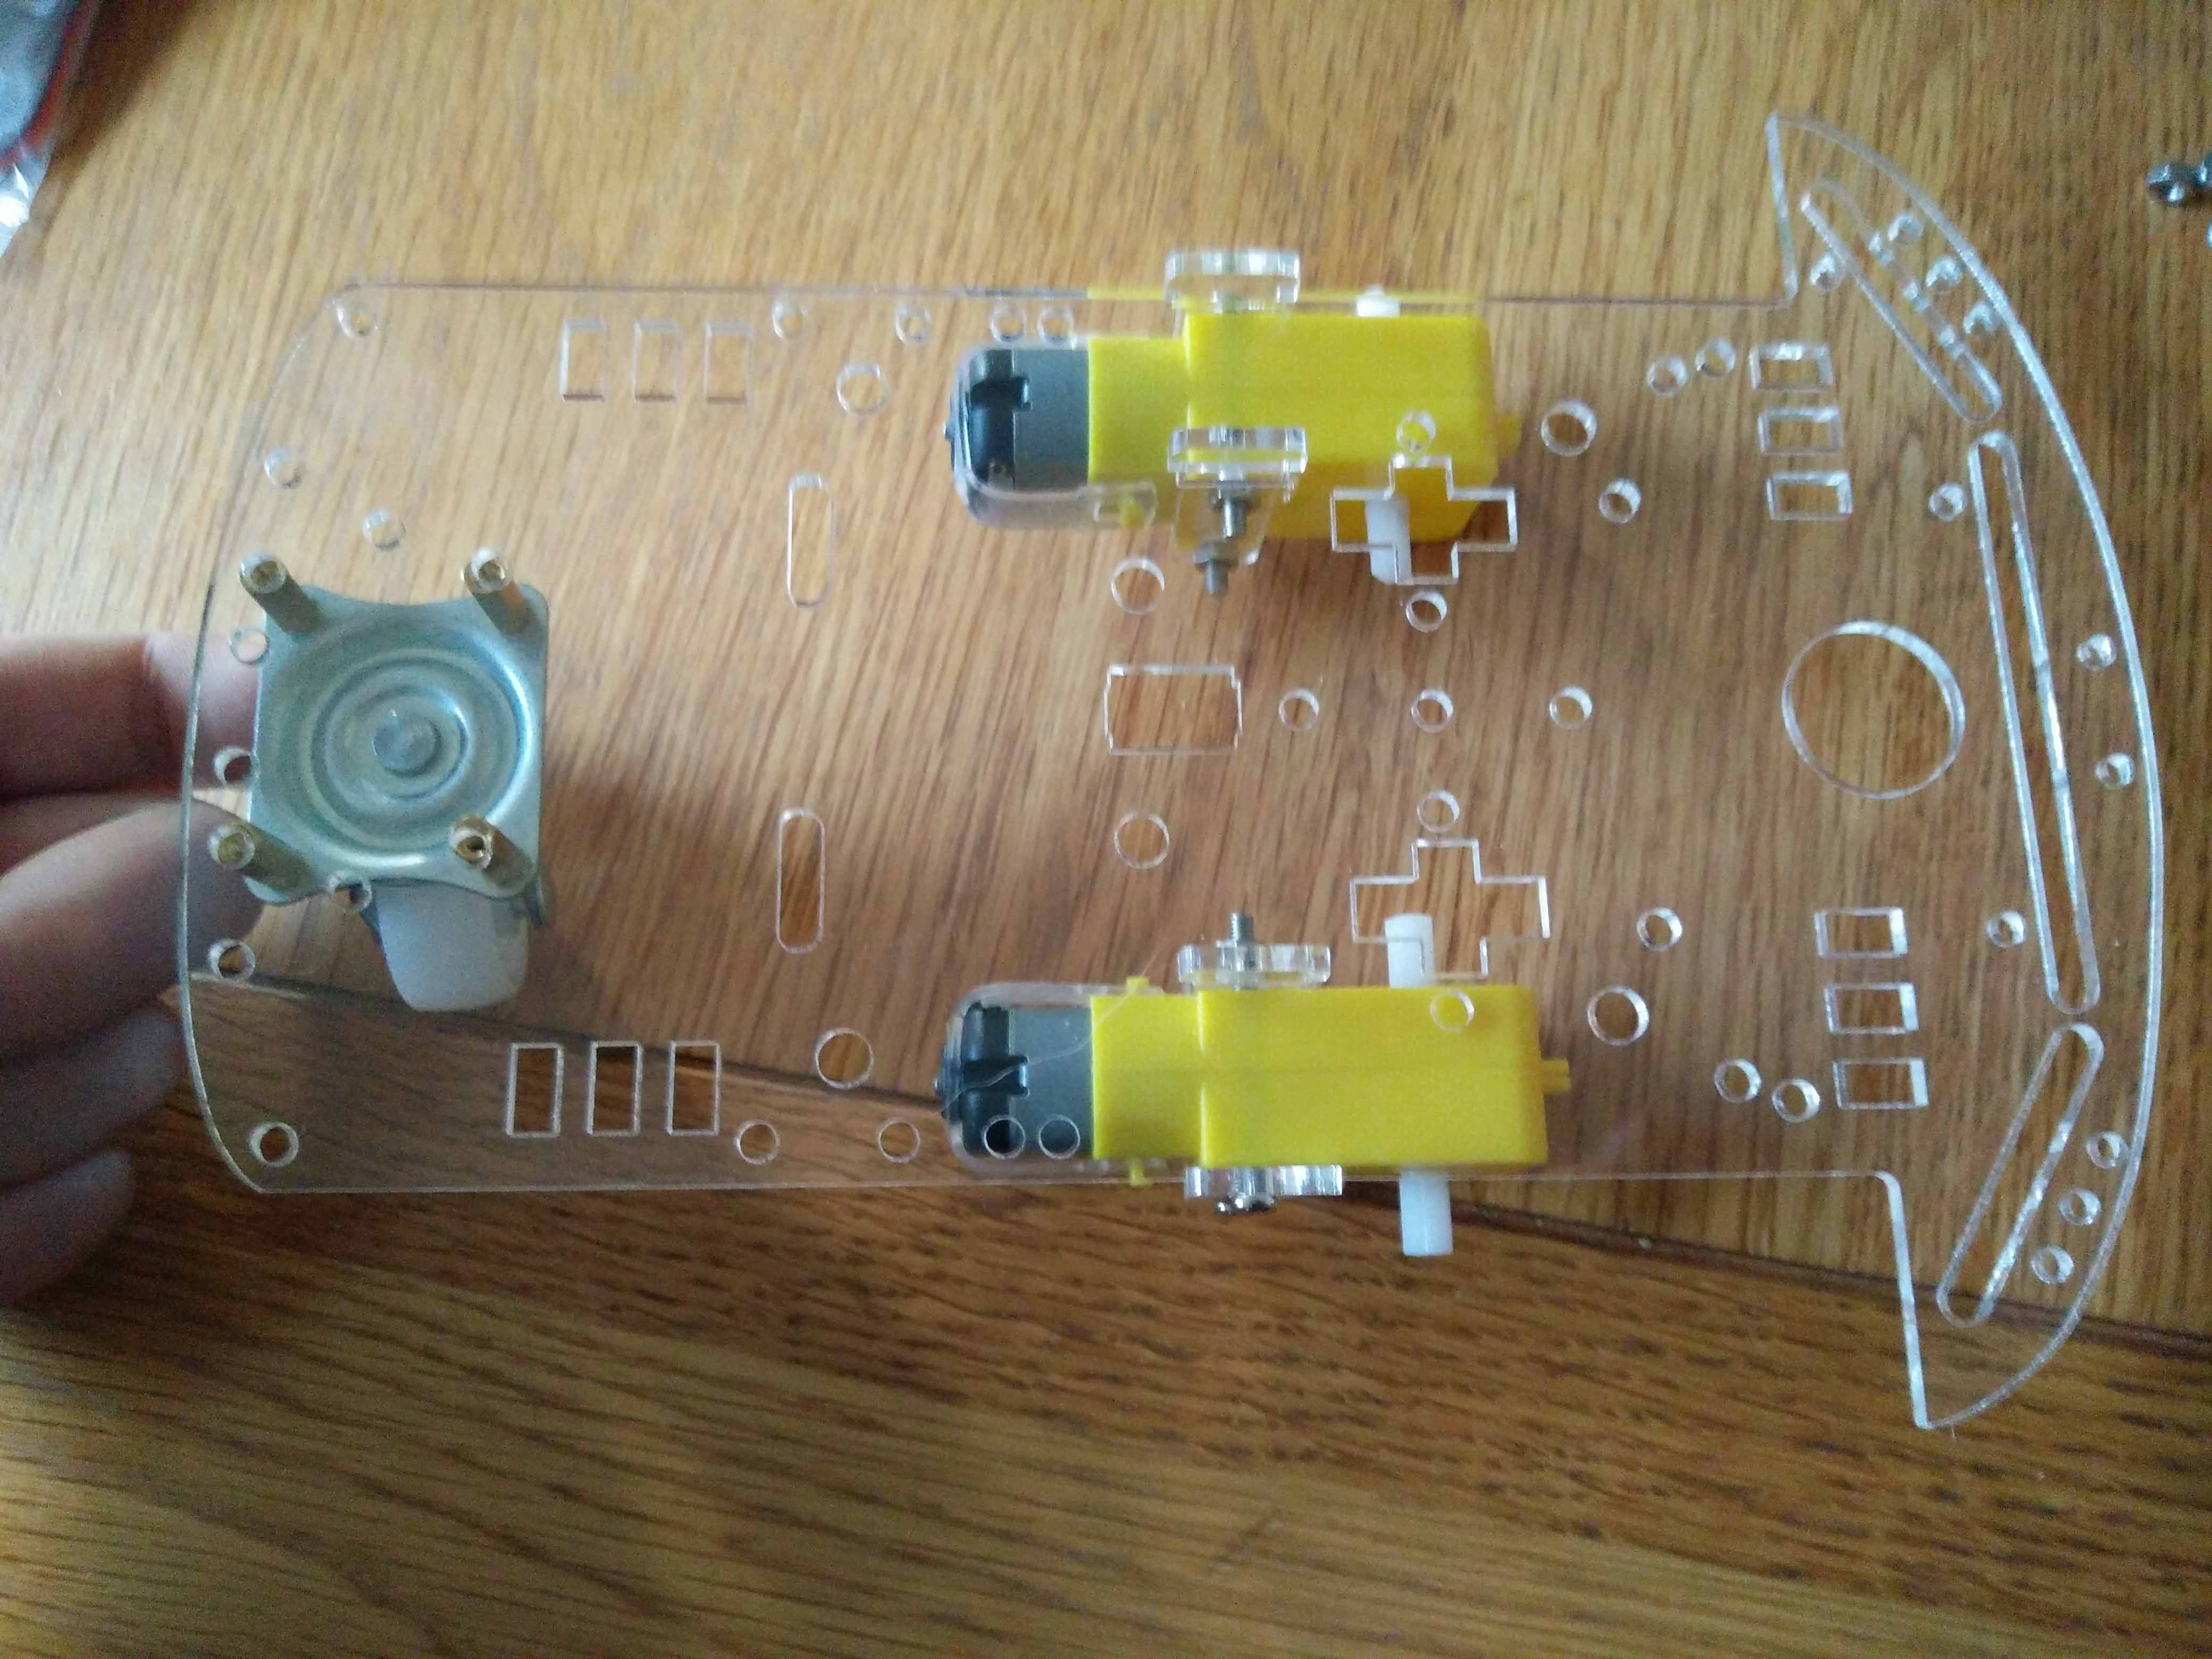
\includegraphics[width=15cm]{img/9.jpg}\par
    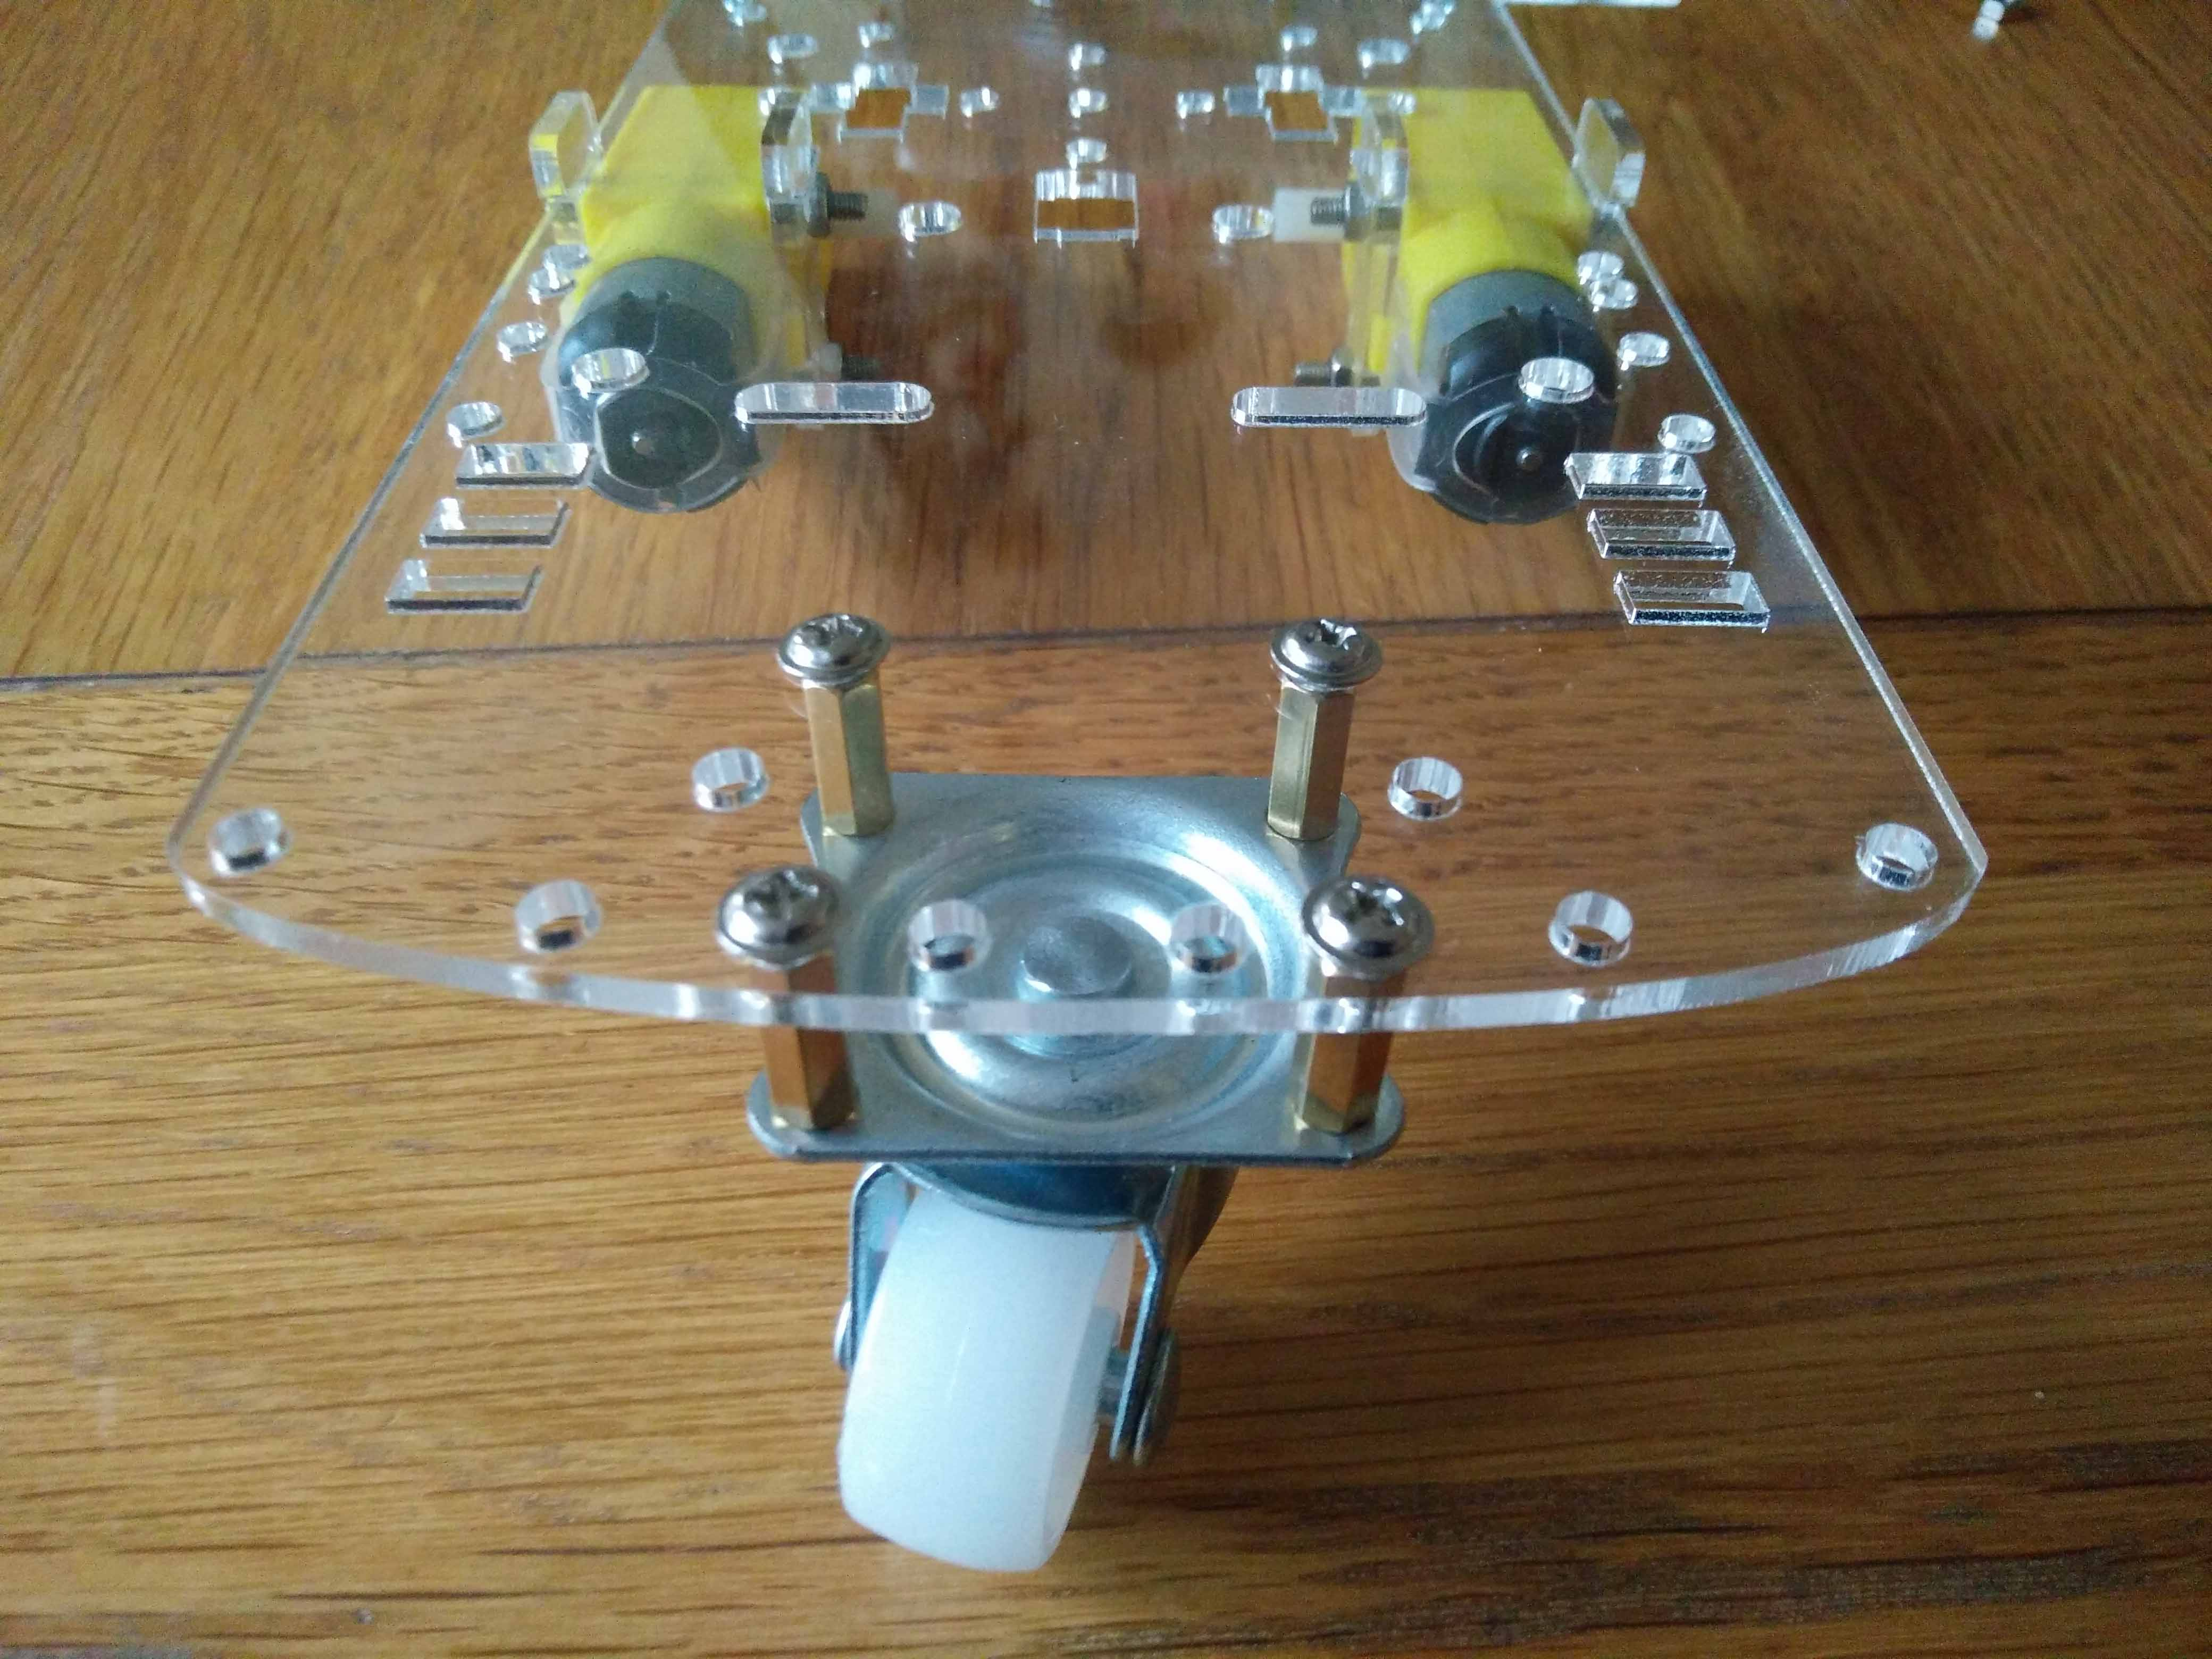
\includegraphics[width=15cm]{img/10.jpg}\par
    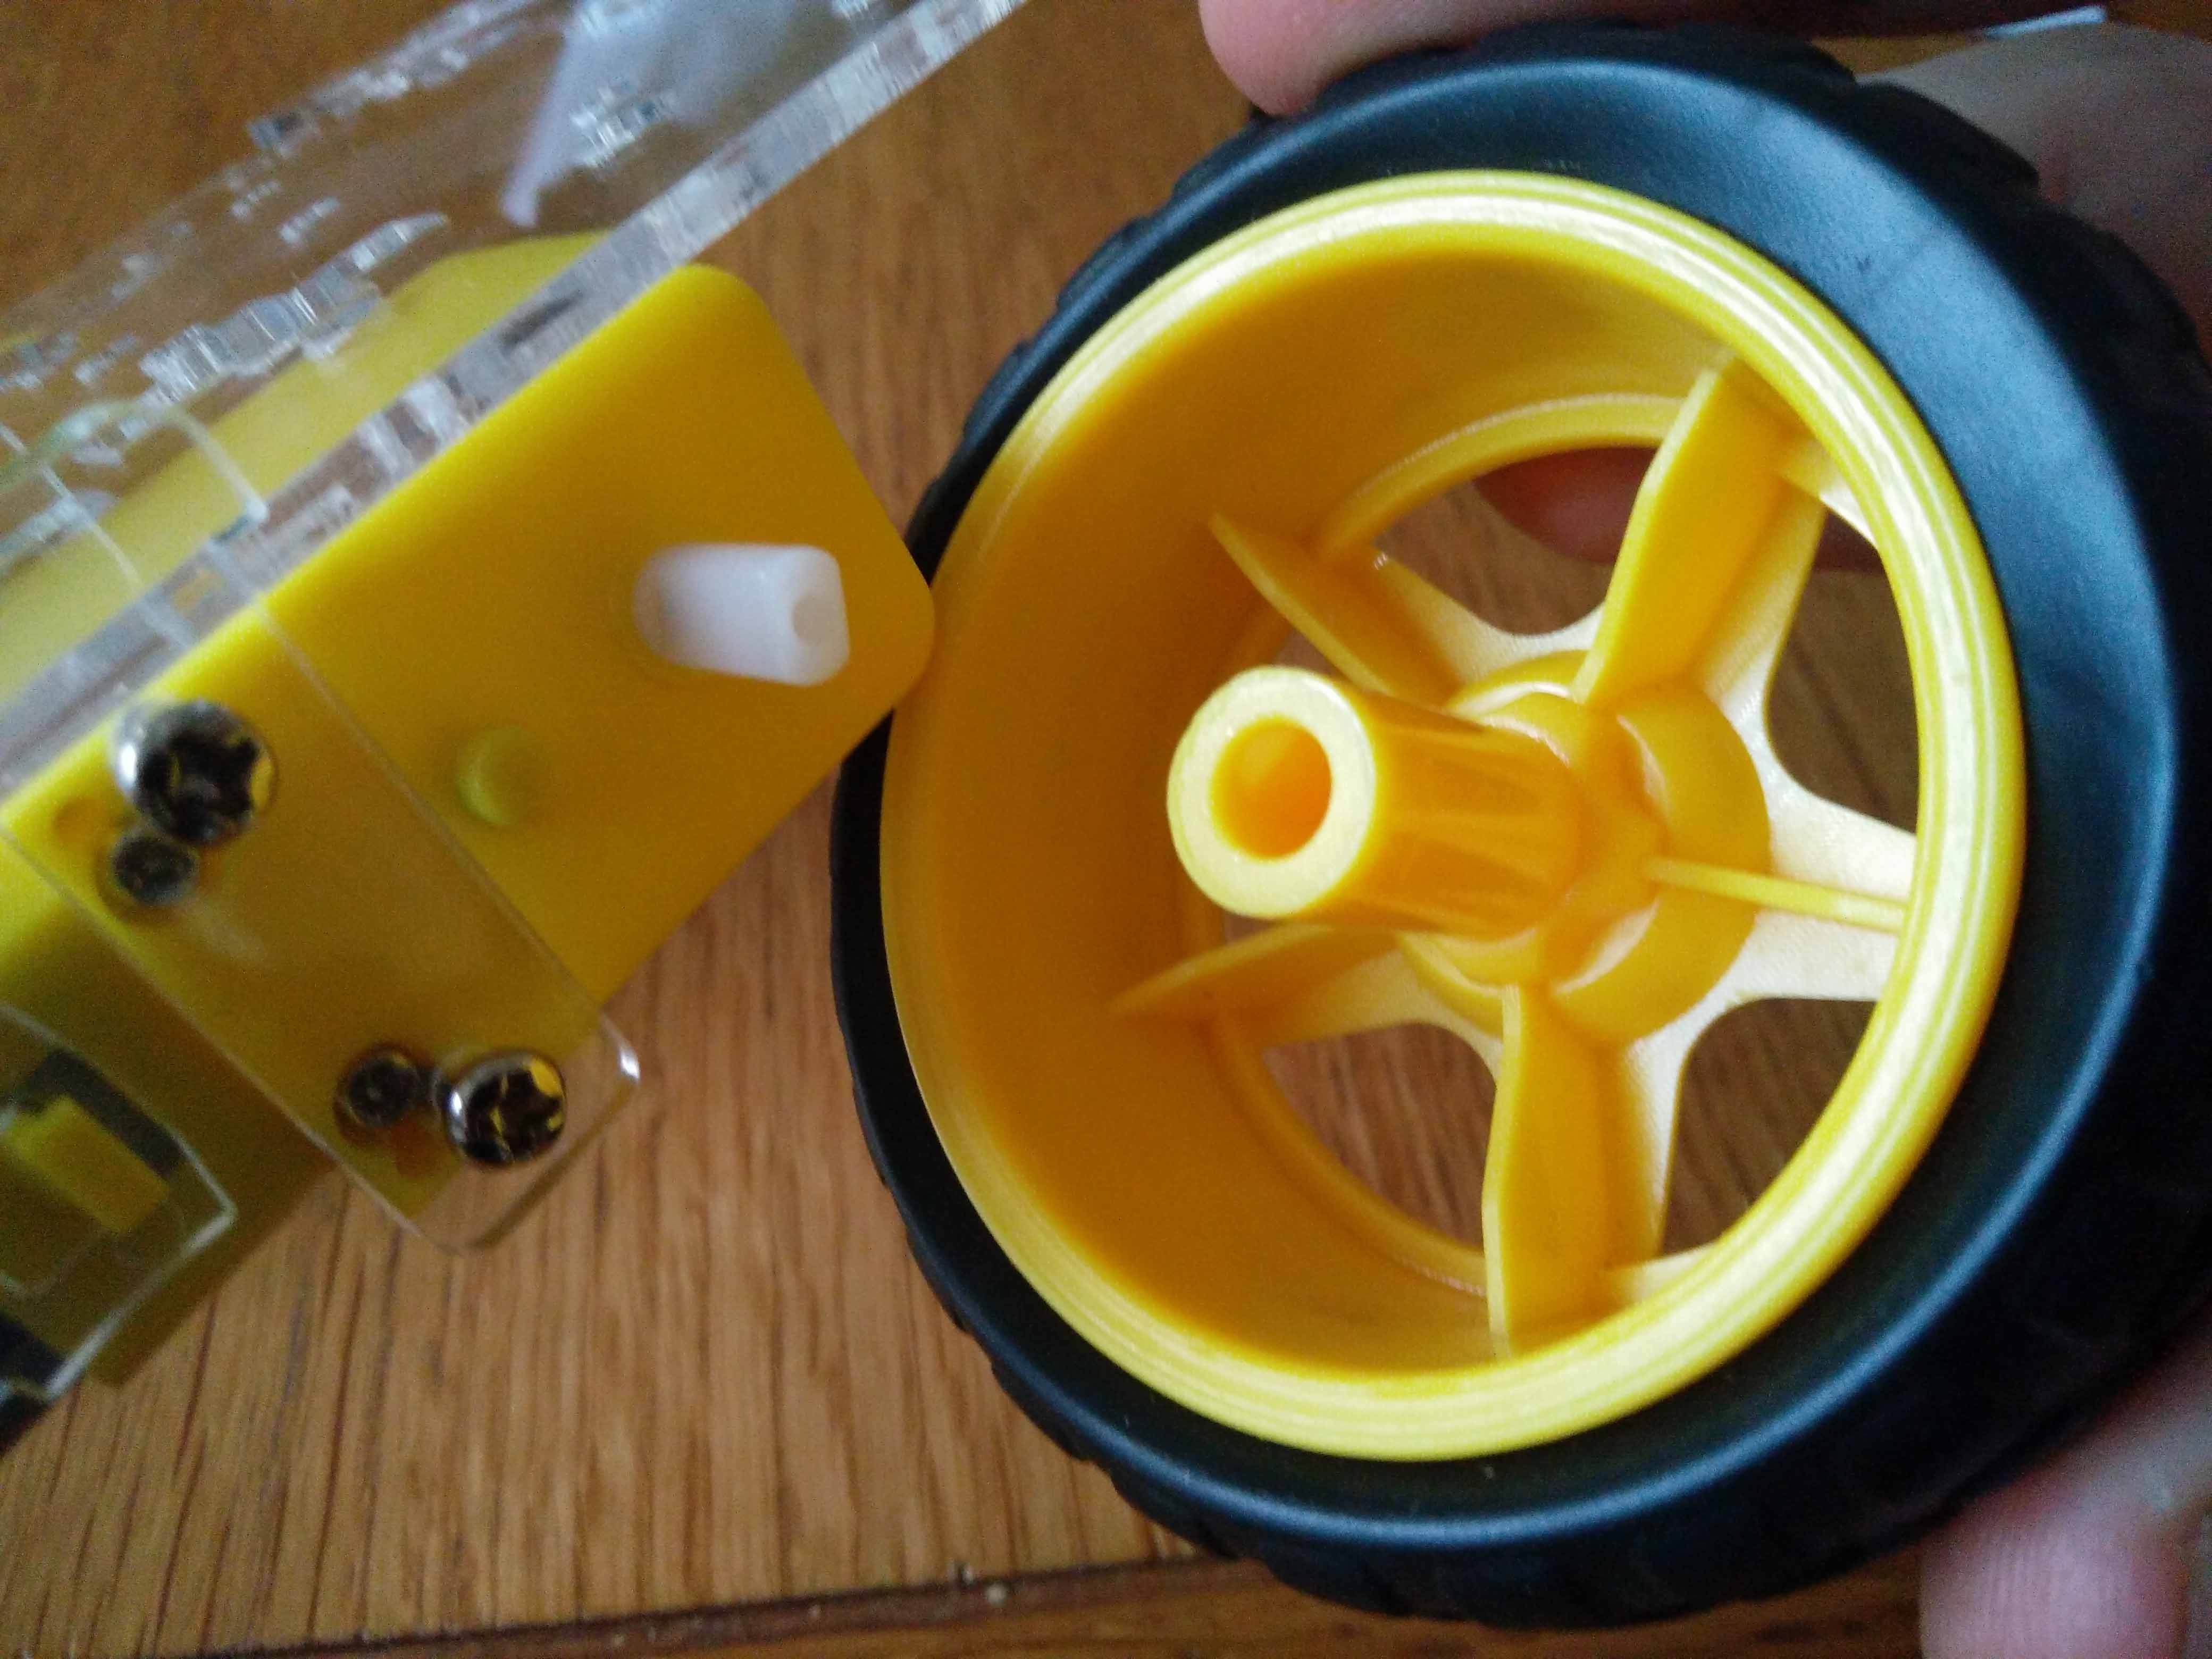
\includegraphics[width=15cm]{img/11.jpg}\par
    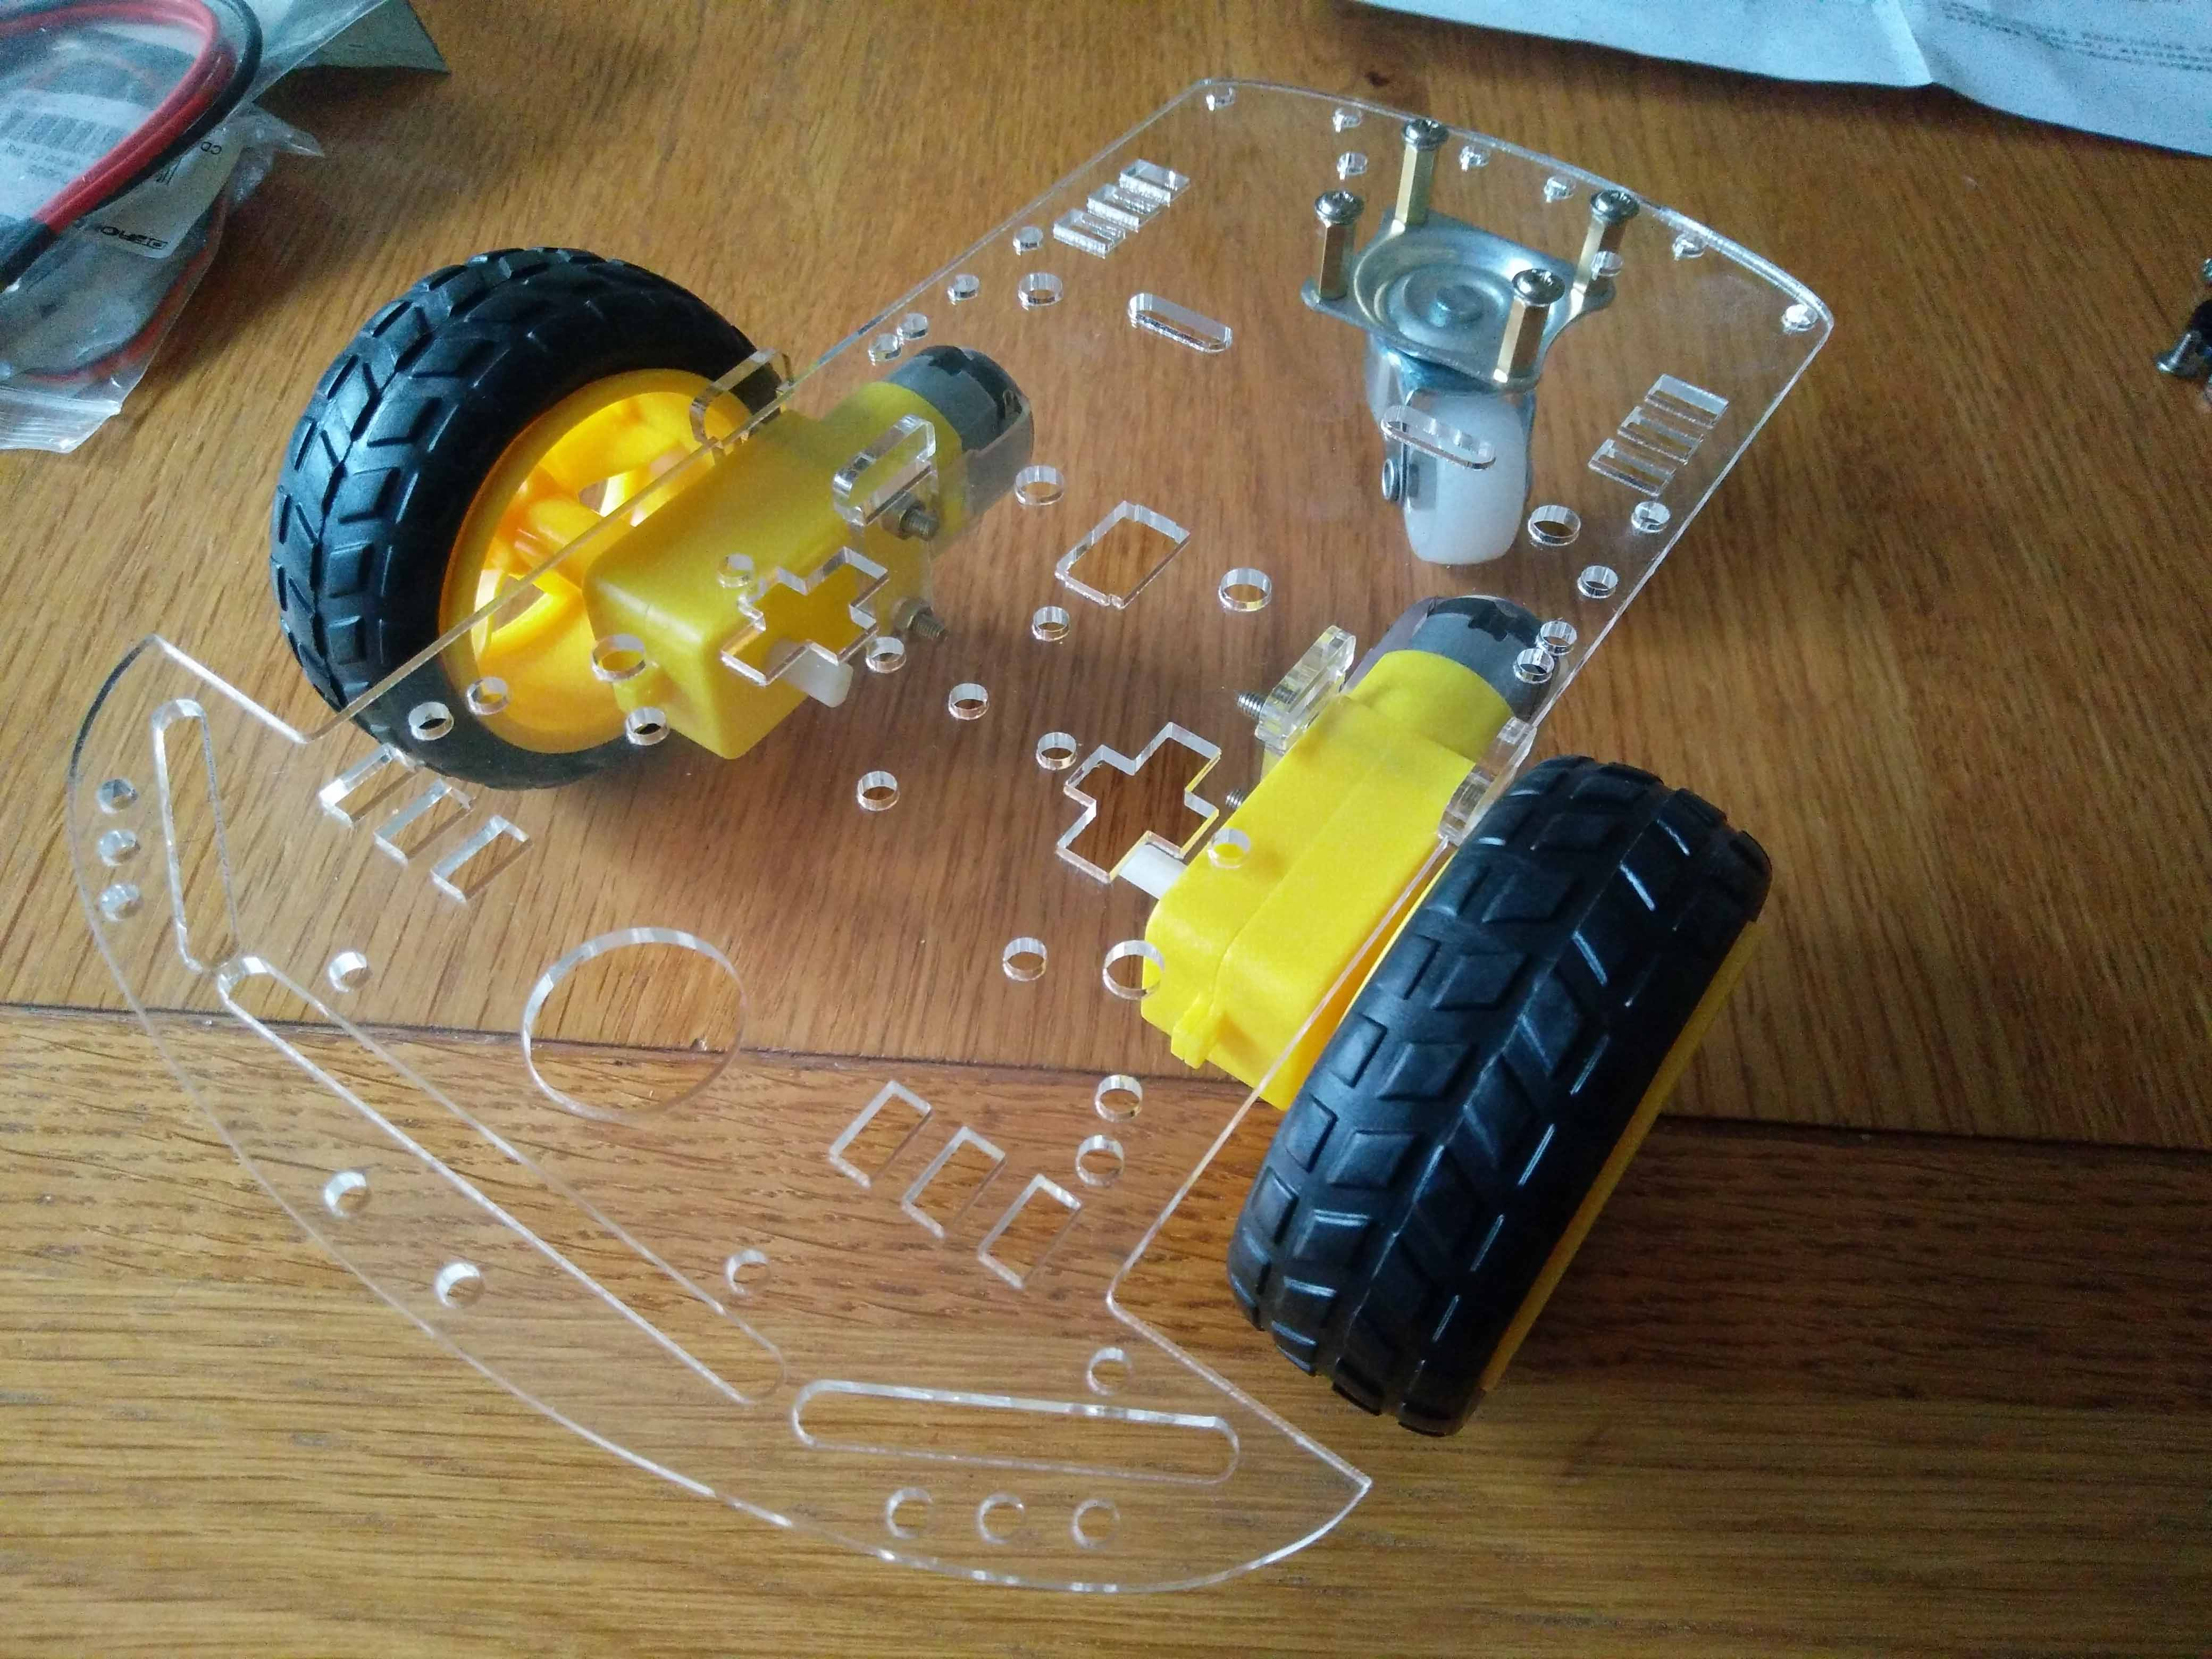
\includegraphics[width=15cm]{img/12.jpg}

    \end{document}